% !TEX TS-program = pdflatex
% !TEX encoding = UTF-8 Unicode
\documentclass[12pt,
    driverfallback=dvipdfm,
 %   openright,
 	openany,
    a4paper,
 %   parskip=half,   
    toc=bibliography,
    twoside,
    numbers=noenddot]{book}              % Book class in 11 points
    \usepackage[usenames,dvipsnames,showerrors]{xcolor}
    \usepackage[
    driverfallback=dvipdfm,
    colorlinks,
    linkcolor=blue,
    citecolor=blue,
    urlcolor=black,
    bookmarks=true
    ]{hyperref}
    
\usepackage{logicproof}
\usepackage{fancyhdr}
%\usepackage{mathptmx}
\usepackage{makeidx}
\makeindex

\usepackage{sidecap}
\usepackage{float}
\floatstyle{ruled}
\newfloat{problem}{thp}{lop}
\floatname{problem}{Problem}
\usepackage{enumitem}
\usepackage{multicol}

%\usepackage{fullpage}
    
%\raggedright                            % do not right justify


\title{\bf Logic for Computer Science}    % Supply information
\author{Sreejith A. V. (sreejithav@iitgoa.ac.in)}              %   for the title page.
\date{IIT Goa, lecture notes}                           %   Use current date. 
%\usepackage{mwe}
%\usepackage{xcolor}
%\usepackage[markcase=noupper]{scrlayer-scrpage}

\pagestyle{fancy}
\fancyhf{}
\fancyhead[LE]{\leftmark}
\fancyhead[RO]{\rightmark}
%\fancyhead[RE,LO]{Guides and tutorials}
\fancyhead[LO]{}
%\fancyfoot[CE,CO]{\leftmark}
\fancyfoot[LE,RO]{\thepage}
 
%\renewcommand{\headrulewidth}{1pt}
%\renewcommand{\footrulewidth}{1pt}
\renewcommand{\chaptermark}[1]{\markboth{\thechapter.\ #1}{}}

%\ohead{}% clear the outer head
%\addtokomafont{pagehead}{\sffamily}
%\addtokomafont{pagefoot}{\tiny}% Making the foot extra tiny to demonstrate
%\addtokomafont{pagenumber}{\normalsize}% that the page number can be controlled on its own. 
%\ofoot*{\pagemark}% the pagenumber in the outer part of the foot, also on plain pages
%\ifoot*{Sreejith\\sreejithav@iitgoa.ac.in}% Name and title beneath each other in the inner part of the foot
%\setlength{\footheight}{24.0pt}

%\documentclass[UKenglish,a4paper,12pt]{article} % use larger type;
%\usepackage[utf8]{inputenc} % set input encoding (not needed with XeLaTeX)
%\usepackage[T1]{fontenc}
%\usepackage{lmodern}

% Author macros::begin %%%%%%%%%%%%%%%%%%%%%%%%%%%%%%%%%%%%%%%%%%%%%%%%
%\title{\mathversion{bold}2. Propositional Logic}
%\author{A. V. Sreejith (IIT Goa)}
%\date{~}

\newcommand\tab[1][1cm]{\hspace*{#1}}

%%% PACKAGES
\usepackage{tikz}
\usetikzlibrary{shapes,arrows, positioning}
\usepackage{algorithm,algorithmic}% http://ctan.org/pkg/algorithms
    
\tikzstyle{decision} = [diamond, draw, fill=yellow!40, 
    text width=4.5em, text badly centered, node distance=1.75cm, inner sep=0pt]
\tikzstyle{decisiong} = [diamond, draw, fill=blue!40, 
    text width=4.5em, text badly centered, node distance=1.75cm, inner sep=0pt]
\tikzstyle{block} = [rectangle, node distance=1.75cm, minimum width=1cm, minimum height=0.5cm, draw, fill=yellow!20, 
    text width=30em, text centered, rounded corners, minimum height=1.5em]
\tikzstyle{blockg} = [rectangle, minimum width=1cm, minimum height=0.5cm, draw, fill=blue!20, 
    text width=15em, text centered, rounded corners, minimum height=1.5em]
\tikzstyle{line} = [draw, -latex']
\tikzstyle{cloud} = [draw, ellipse,fill=yellow!20, node distance=1.5cm, 
    minimum height=2em]
\tikzstyle{invis} = [draw, fill=yellow!10, node distance=4.25cm, 
    minimum height=2em]
\tikzstyle{invisg} = [draw, fill=yellow!10, node distance=3.5cm, 
    minimum height=2em]
\tikzstyle{matheq} = [node distance=8.75cm, text width=21em, minimum width=1cm, 
    minimum height=2em, text centered]

\usepackage{amssymb,amsmath,amsthm}
\usepackage{bussproofs}
\usepackage{caption}
\usepackage{subcaption}

\usepackage{float}
\restylefloat{table}

\newcommand{\chapquote}[3]{\begin{quotation} \textit{#1} \end{quotation} \begin{flushright} - #2, \textit{#3}\end{flushright} }
\newcommand{\myquote}[1]{\begin{quotation} \textit{#1} \end{quotation}}

\newtheorem{theorem}{Theorem}[chapter]
\newtheorem{corollary}{Corollary}[chapter]
\newtheorem{definition}{Definition}[chapter]
\newtheorem{exercise}{Exercise}[chapter]
\newtheorem{example}{Example}[chapter]
\newtheorem{puzzle}{Puzzle}[chapter]
\newtheorem*{solution}{Solution}

\newtheorem{lemma}[theorem]{Lemma}
\newtheorem{claim}[theorem]{Claim}


\newcommand{\true}{T}
\newcommand{\false}{F}
\newcommand{\ifthen}{\Rightarrow}
\newcommand{\ifonlyif}{\Leftrightarrow}
\newcommand{\xor}{\oplus}
\newcommand{\proves}{\vdash}
\newcommand{\andintro}{\wedge i}
\newcommand{\andelim}[1]{\wedge e_{#1}}
\newcommand{\doublenegelim}{\neg\neg e}
\newcommand{\doublenegintro}{\neg\neg i}
\newcommand{\implelim}{\ifthen e}
\newcommand{\implintro}{\ifthen i}
\newcommand{\orintro}[1]{\vee i_{#1}}
\newcommand{\orelim}{\vee e}
\newcommand{\negintro}{\neg i}
\newcommand{\negelim}{\neg e}
\newcommand{\falseelim}{\false e}
\newcommand{\Nat}{\mathbb{N}}
\newcommand{\nmodels}{\not \models}
\newcommand{\nproves}{\not \vdash}
\newcommand{\etal}{\emph{et al.}}
\newcommand{\wall}{~|~}
\newcommand{\defs}{::=}

\newcommand{\indexit}[1]{\emph{#1} \index{#1}}


\begin{document}
\frontmatter                            % only in book class (roman page #s)
\maketitle                              % Print title page.
\tableofcontents                        % Print table of contents
\mainmatter                             % only in book class (arabic page #s)
\chapter*{Notations}
\begin{enumerate}
\item $p,q, p_1,p_2,\dots$ (small letters) - propositional symbols
\item $\alpha, \beta, \gamma, \dots $ (small greek letters) - formulas
\item $\Gamma, \Delta, \Psi \dots$ (capital greek letters) - sets of formulas
\end{enumerate}

\part{Mathematical Tools}
\chapter{Introduction}
We require the following mathematical concepts to understand the lecture notes. The notions of sets, cardinality of sets (countable, uncountable), functions, relations, trees, binary trees, infinite trees, parse trees, graphs, mathematical induction, structural induction. We would also be using notions from computational complexity perspective like Non-deterministic polynomial time (NP), NP-hard, NP-complete, undecidability etc.
%\chapter{Computational Complexity}

%\chapter{Counting and Probability}
%\section{Introduction to Probability}
%\section{Markov Chains}

\chapter{Set Theory}
\section{Mathematical Induction}
\label{chap:mathInd}

Consider a property which is true for every natural number. We will denote by $P(n)$ the fact that the property is true for the number $n$. For example
\begin{enumerate}
\item $P(n):$ The sum of numbers from $1$ to $n$ is $\frac{n(n+1)}{2}$. 
\item $P(n):$ The sum of numbers from $1$ to $n^2$ is $\frac{n(n+1)(2n+1)}{6}$.
\item $P(n):$ There is a prime number greater than $n$.
\end{enumerate}

We can use mathematical induction to prove the correctness of such properties. There are three components in mathematical induction. 
\begin{enumerate}
\item Induction Hypothesis (IH): This is the property, $P(n)$ we are interested in proving, for all $n \in \Nat$. In many cases we will have to restate the theorem statement in a way suitable for induction. For example, the statement, ``there are infinite number of primes" can be rephrased as ``For all $n$, there is a prime number greater than $n$".
\item Base case: In the base case, we show that the theorem statement (in other words $P(n)$) is true for the smallest $n$. In the case of all the examples above, the least number for which $P(n)$ is true is $n=1$. There might be cases when the base case need not be $1$. There are certain situations, when the base case consists of more than $1$ case.
\item Inductive step: In the inductive step, we first assume that the statement $P(n)$ is true and show that $P(n+1)$ is true. In a stronger version of induction, we assume that $P(k)$ is true for all numbers $k \leq n$. Using this assumption we show that $P(n+1)$ is true.
\end{enumerate}

The statement of weak mathematical induction can be expressed using the following equivalence statement (understanding the following expression will require knowing first order logic).
\[
\Big(P(1) \wedge \forall n ~\big(P(n) \implies P(n+1)\big)\Big) \implies \forall x ~P(x)  
\]

Let us look at an example now.
\begin{theorem}
The number of subsets of an $n$ element set is $2^n$.
\end{theorem}
\begin{proof}
The induction hypothesis is the following.

\centerline{For all $n \geq 0$, the number of subsets of an $n$ element set is $2^n$.}
We now show that the theorem is true for the base case. \\
Base case ($n=0$): The only subset of a $0$ element set (empty set) is the empty set itself. \\
Inductive step: Let us assume that the claim is true for an $n$ element set. That is the number of subsets is $2^n$. Now let us consider an $n+1$ element set. Without loss of generality we can assume the set is $\{1,2,\dots,n+1\}$. We can now partition the set of all subsets into two parts. $(1)$ All sets without element $n+1$. and $(2)$ all sets with the element $n+1$. By induction hypothesis, the first part consists of $2^n$ elements (the set of all subsets of $\{1,2,\dots,2^n\}$). Each subset in the second part can be created by taking a subset from the first part and inserting the $n+1$ element. Therefore this part also consists of $2^n$ elements. Hence the total number of subsets of $n+1$ elements is $2^n + 2^n = 2 \times 2^n = 2^{n+1}$.
\end{proof}

One has to be extremely careful while designing a proof by induction. All arguments we make in the inductive step should necessarily hold for all values of $n$. Otherwise we can fall into traps, proving statements which are false. Here is an example of a wrong use of induction hypothesis. Readers are requested to find out what is wrong in the proof.
\begin{example}
What is wrong in the following proof by induction. 

We prove using induction that

\centerline{``For all classes of size $n$, either everyone is male or everyone is female."}

Base case ($n=1$): For a class of size $1$, the claim is obviously true.

Inductive step: Let us assume the claim holds for all classes of size $n$. Consider a class $\{1,2,\dots,n,n+1\}$ of size $n+1$.  From induction hypothesis, it follows that in the class of $\{1,2,\dots,n\}$ either all are male or all are female. That is the persons $1$ and $n$ have the same gender. Using induction hypothesis again, the class of $\{1,2,\dots,n-1,n+1\}$ also has either all male or all female. This gives us that $1$ and $n+1$ is of the same gender. Therefore our claim holds for the class $\{1,2,\dots,n+1\}$. 
\end{example}

\begin{exercise}
Prove using induction hypothesis the following
\begin{enumerate}
\item $1+2+\dots+n = \frac{n(n+1)}{2}$.
\item $1^2+2^2+\dots+n^2 = \frac{n(n+1)(2n+1)}{6}$.
\item The pigeon hole principle
\end{enumerate}
\end{exercise}

\begin{exercise}
Prove the equivalence between mathematical induction and strong mathematical induction.
\end{exercise}


\part{Propositional Logic}
% !TeX root = logicNotes.tex

\chapter{Introduction to Propositional Logic}
\section{Declarative statements}
We are interested in creating a language in which mathematical proofs can be written. The language should be simple enough so that vague and unambiguous statements cannot be written. On the other hand, it should be powerful enough for proofs to be written. We will build a language in which all of mathematics can be embedded. We begin with propositional logic, the foundation on which other logics are built on.

We say that \emph{true} and \emph{false} are \emph{boolean values}. They will be denoted by the symbols \true\/ and \false\/ respectively. \indexit{Declarative sentences} are statements which can be assigned either true or false. For example,
\begin{enumerate}
\item 179179 is a composite number.
\item Sun rises in the east and Japan is in Europe
\item Kattapa killed Bahubali.
\item P = NP
\item John Snow's father is Ned Stark
\end{enumerate}
Since the number 179179 is divisible by 7,11,13 and 179, statement (1) is true. On the other hand statement (2) is false since Japan is not in Europe. Statement (3) is true. We do not yet know whether Statement (4) is true or false but the statement as such can be assigned true or false. Statement (5) is true or false depending on till which episode you have watched game of thrones. 

The following statements are not declarative 	
\begin{enumerate}
\item What is the time?
\item Submit your assignments today.
\item Teek Hai!
\end{enumerate}

Some declarative statements can be thought of as \indexit{atomic}. That is, those statements cannot be further split into logical sentences. In the above example Statement (2) is not atomic because it can be split into sentences ``Sun rises in the east'' and ``Japan is in Europe''.

\section{Propositions}
As mathematicians we are not interested in the information contained in the declarative sentences. That is, we are not interested whether ``Kattapa killed Bahubali" or ``Sun rises in the east" in the real world. Rather we are interested in only whether the statements are true or false and what other statement can we understand from them. For example, consider the following statement.

\myquote{``If it rains in Delhi today, you will fail in logic course."}

This is a weird statement but the statement is a declarative statement. That is, it can either be true or false. To summarize the point being made. We are not really interested in the weirdness or the reality of the real world. We are only interested in statements which can be assigned boolean values. Hence we map declarative sentences to symbols. We will denote atomic sentences using symbols $p,q,r,\dots$ or $p_1,p_2,\dots$. These will be termed as \indexit{propositions} and the logic we build using propositions as \emph{propositional logic}. We will also denote true by \true\/ and false by \false.

Propositions can be modified/combined using certain symbols called \indexit{logical connectives}. This way we can build complex logical statements. The logical connectives we will be interested in and their \indexit{semantics} follow
\paragraph{Negation} \index{negation} For any sentence, its negation is the opposite of it. For example, the negation of ``Kattapa killed Bahubali'' is ``Kattapa did not kill Bahubali''. Similarly negation of ``P=NP'' is ``P $\neq$ NP''. The negation of a propositional symbol, $p$ is denoted as $\neg p$ (and called negation of $p$). If the $p$ is true then $\neg p$ is false. On the other hand, if $p$ is false, $\neg p$ is true. The following \indexit{truth table} summarizes the semantics of negation.

\begin{table}[ht]
\centering
\begin{tabular}{c|c}
$p$ & $\neg p$ \\
\hline
\true & \false \\
\false & \true \\
\end{tabular}
\caption{Truth table for negation}
\end{table}

\paragraph{Conjunction} \index{conjunction} stands for \emph{and}. When it is used to connect two declarative sentences it means that both the sentences are true. 
For example, ``$2$ is a prime number'' and ``$2$ is an even number''. We use the symbol $\wedge$ to denote and. The following truth table captures the meaning of $\wedge$.

\begin{table}[H]
\centering
\begin{tabular}{c|c|c}
$p$ & $q$ &$p \wedge q$ \\
\hline
\true & \true & \true \\
\true & \false &  \false \\
\false & \true & \false \\
\false & \false & \false 
\end{tabular}
\caption{Truth table for conjunction}
\end{table}


\paragraph{Disjunction} \index{disjunction} stands for \emph{or}. Disjunctions are slightly different from the or we use in English (or most natural languages). Assume that I made the following announcement in class.

\myquote{``Tomorrow there will be a lecture or an exam."}

It is natural for you to assume that there will either be a lecture tomorrow and no exam, or there will be an exam and no lecture. That is, you would never think of the possibility of both a lecture and an exam going to be held tomorrow. But, or used in a mathematical sentence, can mean both of them happening. This is the difference of disjunction in or in logic and natural language. We have a name for the or in natural language. We call it xor and is denoted by the symbol $\xor$. See Exercise \ref{exercise:xor}. Coming back to disjunction in logic, the symbol for or is $\vee$ and its semantics is given by the following truth table.
\begin{table}[H]
\centering
\begin{tabular}{c|c|c}
$p$ & $q$ &$p \vee q$ \\
\hline
\true & \true & \true \\
\true & \false &  \true \\
\false & \true & \true \\
\false & \false & \false 
\end{tabular}
\caption{Truth table for disjunction}
\end{table}
The semantics for xor is given below.

\begin{table}[ht]
\centering
\begin{tabular}{c|c|c}
$p$ & $q$ &$p \xor q$ \\
\hline
\true & \true & \false \\
\true & \false &  \true \\
\false & \true & \true \\
\false & \false & \false 
\end{tabular}
\caption{Truth table for xor}
\end{table}


\paragraph{Implication} \index{implication} is used to state a necessary condition. It is denoted by the symbol $\ifthen$. The statment 
\myquote{If $x$ is prime, then $x \neq 4$}
 is an example of an implication. Typically it is written in the form ``If $p$ then $q$'' and in propositional logic as $p \ifthen q$.  Its truth table is given in Table \ref{tab:implication}.
\begin{table}[ht]
\centering
\begin{tabular}{c|c|c}
$p$ & $q$ &$p \ifthen q$ \\
\hline
\true & \true & \true \\
\true & \false &  \false \\
\false & \true & \true \\
\false & \false & \true 
\end{tabular}
\caption{Truth table for implication}
\label{tab:implication}
\end{table}
We will explain the truth table with an example. Consider the statement 

\myquote{``If you work hard, you get good grades''. }

The statement is true if you work hard and got good grade. On the other hand it is false if you work hard and did not get good grades. The tricky question is, what if you did not work hard and got good grades. Does this violate our the statement? No, it doesnt and hence we can assign the statement to be true in this case also. Similarly the statement is true, if we did not work hard and did not get good grades.

Implication is a little tricky to understand especially for beginners. The following puzzle helps you to understand it better.
\begin{puzzle}[Wason]
The following cards are kept on the table. Each card has a letter on one side and a number on the other side.
\begin{figure}[h]
\centering
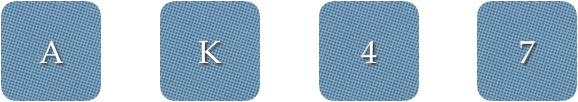
\includegraphics[width=8cm]{ak47.jpg}
\end{figure}
We make the following claim: ``If a card has a vowel on one side, then it has an even number on its opposite side". Which cards must one flip to check if the claim is correct?
\end{puzzle}
\begin{solution}
The answer is cards $A$ and $7$. Let us look at each of the card and check whether we need to flip or not. Card A has to be flipped, because we need to be sure that on the opposite side is a vowel. Card K need not be checked. Why? Because, it does not matter to us if, the opposite side has an even number or odd number. Similarly we do not have to flip $4$ since it does not matter to us whether the opposite side was vowel or consonant. On the other hand, card $7$ has to be flipped because we have to make sure it is not a vowel on the other side. Because if there was a vowel, we would have violated the claim.
\end{solution}

\section{Formulas}
By repeatedly using logical connectives we can make complex declarative statements. For example, 

\myquote{If $x$ is prime and $x \neq 2$,  then $x$ is odd}

is a statement made by first conjuncting two statements ``$x$ is prime" and ``$x \neq 2$". It is then used in implication with statement ``$x$ is odd". In propositional logic this statement can be wrriten as follows
\myquote{$($``$x$ is prime" $\wedge$ ``$x \neq 2$"$) \ifthen$ ``$x$ is odd"}
Such complex statements in logic are called \indexit{formulas}. We denote propositional formulas by greek letters like $\alpha, \beta, \gamma, \dots$ etc or $\alpha_1, \alpha_2, \dots$.
\begin{definition}
A {formula} is inductively constructed using the following rules (and no other rules)
\begin{enumerate}
\item A proposition is a formula
\item If $\alpha$ and $\beta$ are formulas then $\neg \alpha$, $\alpha \vee \beta$, $\alpha \wedge \beta$, $\alpha \ifthen \beta$ are formulas
\end{enumerate}
\end{definition}
We can write truth tables for formulas by inductively building the table. Consider the following formula and its truth table $$\alpha \defs \big((p \ifthen \neg q) \ifthen (q \vee \neg p)\big)$$.
\begin{table}[H]
\centering
\begin{tabular}{c|c|c|c|c|c|c}
$p$ & $q$ &$\neg p$ & $\neg q$ & $p \ifthen \neg q$ & $q \vee \neg p$ & $\alpha$ \\
\hline
\true & \true & \false & \false & \false & \true & \true \\
\true & \false &  \false & \true & \true & \false & \false \\
\false & \true & \true  & \false & \true & \true & \true \\
\false & \false & \true & \true & \true & \true & \true
\end{tabular}
\caption{Truth table for $\alpha \defs \big((p \ifthen \neg q) \ifthen (q \vee \neg p)\big)$}
\end{table}


For a formula $\alpha$ with propositions $p_1,p_2,\dots, p_n$, a \indexit{valuation} is a particular \true/\false\/ assignment to the propositions $p_1,\dots, p_n$. That is a valuation, $v: \{p_1,p_2,\dots,p_n\} \rightarrow \{\true, \false\}$ is a function from the propositions to boolean values. Note that, there are $2^n$ different valuations possible for $n$ propositions.
\begin{example}
Consider the formula $p \wedge q$. One particular valuation is $p$ is assigned \true\/ and $q$ is assigned \false. The formula is evaluated to false for this valuation.
\end{example}

%\section[Types of Formulas]{Types of Formulas: Tautology, Contradiction, \dots}
We say that two formulas are \indexit{equivalent} if they have the same truth table. It will be denoted by the symbol $\equiv$. \index{$\equiv$} 

\begin{example}
If and only if (written also as \indexit{iff}) is used to denote a necessary and sufficient condition. In symbolic form it is denoted by $\ifonlyif$. Semantically $p \ifonlyif q$ is equivalent to $p \ifthen q$ and $q \ifthen p$. The truth table is given below.
\begin{table}[H]
\centering
\begin{tabular}{c|c|c}
$p$ & $q$ &$p \ifonlyif q$ \\
\hline
\true & \true & \true \\
\true & \false &  \false \\
\false & \true & \false \\
\false & \false & \true 
\end{tabular}
\label{tab:iff}
\caption{Truth table for if and only if}
\end{table}
\end{example}

Here is another example which introduces the \indexit{contrapositive} of an implication. The formula $(\neg q \ifthen \neg p)$ is the {contrapositive} of the statement $p \ifthen q$. The following exercise shows that an implication and its contrapositive are equivalent.
\begin{exercise}
Show that the following formulas are equivalent.
\begin{enumerate}
\item $p \ifthen q$
\item $(\neg q \ifthen p)$
\item $\neg p \vee q$
\end{enumerate}
What is the complement of $p \ifthen q$?
\label{exercise:implequiv}
\end{exercise}


\begin{exercise}[DeMorgan's law]
\label{exercise:demorgansem}
Show that $p \wedge q  \equiv \neg (\neg p \vee \neg q)$ and  $p \vee q  \equiv \neg (\neg p \wedge \neg q)$
\end{exercise}

The following exercise connects xor and disjunctions.
\begin{exercise}
\label{exercise:xor}
Write a formula using only the symbols disjunctions and negations which is equivalent to $p \xor q$.
\end{exercise}

\begin{exercise}
Consider you are given a truth table with propositions $p_1,\dots,p_n$. Give an algorithm which outputs a formula (using only symbols $\vee,\wedge, \neg$) having the same truth table.
\end{exercise}

The above exercise (along with demorgan's law) show that any formula can be converted into an equivalent formula which uses only the symbols $\wedge$ and $\neg$.

\begin{exercise}
Convert any formula into an equivalent formula which uses only symbols $\wedge$ and $\neg$.
\end{exercise}

We say that a formula $\alpha$ is \indexit{satisfiable} if there is a valuation which makes $\alpha$ true. In other words, $\alpha$ is satisfiable if we can find atleast one \true\/ in the column for $\alpha$ in the truth table of $\alpha$. A formula $\alpha$ is a \indexit{tautology} if for all valuations $\alpha$ is true. In other words $\neg \alpha$ is not satisfiable. On the other hand, $\alpha$ is a \indexit{contradiction} or \indexit{unsatisfiable} if $\alpha$ is not satisfiable. That is $\neg \alpha$ is a tautology.
\begin{exercise}
\begin{enumerate}
\item Give a formula which is a tautology?
\item Give a formula which is satisfiable but not a tautology?
\item Give a formula which is a contradiction?
\end{enumerate}
\end{exercise}

\section[Encoding using logic]{Application of Logic: Encoding problems}
We use propositional logic to encode different problems.

\subsection{Digital circuits}
\begin{exercise}
We can view a proposition being assigned to $1$ or $0$ (in place of \true\/ or \false). That is a proposition $p$ can be thought of as a bit variable. Extending the idea, a valuation to a $n$ proposition symbols can be thought of as an $n$-bit number. Use this view to write a formula to encode addition relation between two $n$-bit numbers. That is, write a formula which satisfies the following condition
\begin{align*}
p_1p_2\dots p_n  \\
+ \\
q_1q_2 \dots q_n &  \\
= \\
r_1r_2 \dots r_n
\end{align*}
View $p_1,\dots,p_n,q_1,\dots,q_n,r_1,\dots,r_n$ as propositions.
\end{exercise}

\subsection{Mathematical statements}
\begin{exercise}[Pigeon hole principle]
If $n+1$ pigeons are placed on $n$ holes, atleast one hole will have more than one pigeon. This is the pigeon hole principle. Now, consider $n+1$ pigeons and $n$ holes. Let proposition $p_{i,j}$ denote the fact that the $i^{th}$ pigeon is in the $j^{th}$ hole.  Write a propositional logic formula to encode the pigeon hole principle. 
\end{exercise}


\subsection{Puzzles}
\begin{exercise}[Smullyan]
Use propositional logic to answer the following questions
\begin{enumerate}
\item You are trapped in a room. There are two doors. Either the doors lead to an exit or to a lion (note that both leading to an exit or to a lion are also possible). In Door 1, it is written ``This door is exit and other door leads to lion". In Door 2, it is written ``One of the rooms lead to exit, the other to a lion". You are told that only one of the written statements are true and the other false. Which door would you choose?
\item Similar to the previous question. You are trapped in a room. There are two doors. Either the doors lead to an exit or to a lion (note that both leading to an exit or to a lion are also possible). In Door 1, it is written ``Atleast one of the doors is an exit". In Door 2, it is written ``There is a lion on the other door". You are told that either both are true statements or both are false. Which door would you choose?
\item One more question with same flavour. You are trapped in a room. There are two doors. Either the doors lead to an exit or to a lion (note that both leading to an exit or to a lion are also possible). In Door 1, it is written ``This door is exit or the other door leads to lion". In Door 2, it is written ``The exit is the other door". The statements are either both true or both false. Which door would you choose?
\end{enumerate}
\end{exercise}

\begin{exercise}[Smullyan]*
Can you think of encoding the following problem in propositional logic such that it has a solution iff the formula is satisfiable.
\begin{figure}[H]
\centering
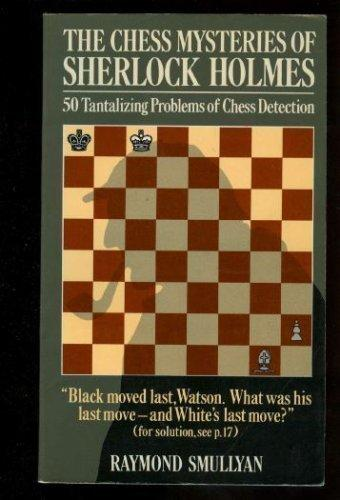
\includegraphics[width=5cm, height=5cm]{chess.jpg}
\end{figure}
The reader is expected to understand how to go about doing this. He/she is not expected to write the entire formula (which is going to be very big).
\end{exercise}

\begin{exercise}[Indian Puzzle championship 2010]*
Fill in the grid in such a way that every row and every column contains numbers from $(1-5)$ exactly once. Some cells may remain blank. The numbers inside the grid represent the height of
the building in the corresponding cell. The numbers outside the grid represent the number of buildings visible from that direction.
\begin{figure}[H]
\centering
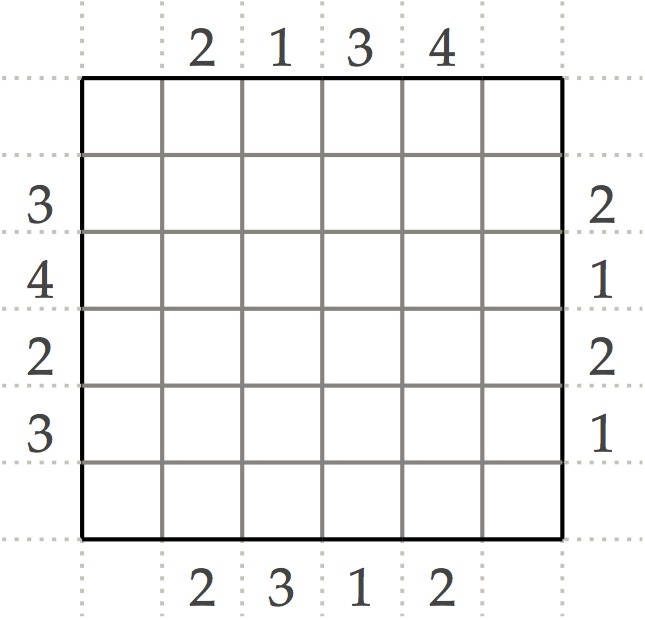
\includegraphics[width=5cm,height=5cm]{skyscrapper.jpg}
\end{figure}

Encode the problem in propositional logic.
\end{exercise}

\section{Satisfiability of propositional formulas}
How hard is it to check whether a propositional formula is satisfiable?  

\begin{problem}
\caption*{{\bf Problem} SAT}
{\bf Input: } A propositional formula $\alpha$ \\
{\bf Output: } YES if $\alpha$ is satisfiable, otherwise NO
\label{prblm:sat}
\end{problem}

For a formula $\alpha$ with $n$ propositions the truth table has $2^n$ number of rows. Therefore building the truth table and checking each row is a trivial way to check for satisfiability. This algorithm though takes exponential time, since the number of rows in the truth table is $2^n$. 
In other words, $O(2^n)$ is an upper bound for checking satisfiability of a formula with $n$ propositions. The interesting question is, does there exist a faster algorithm. Or even better, does there exist a polynomial time algorithm. That is, an algorithm whose number of steps is $O(n^c)$ for some constant $c$. It turns out, we do not yet know the answer to this question. Most computer scientists think there is no polynomial time algorithm for SAT. The problem is NP-complete (in NP and is NP-hard) and hence finding a polynomial time algorithm is equivalent to answering P=NP. 

\begin{exercise}
\label{exercise:satisnp}
Show that SAT is in NP? 
\end{exercise}

To show that SAT is NP-hard, we need to reduce from an NP-complete problem into SAT. The next exercise asks you to reduce from the Hamiltonian problem.

\begin{exercise}
\label{exercise:satisnphard}
Give a polynomial time algorithm which takes as input a graph $G=(V,E)$ and outputs a propositional formula $\alpha$ such that the graph has a Hamiltonian cycle if and only if $\alpha$ is satisfiable. Does the valuation which makes $\alpha$ true give us the cycle? [A Hamiltonian cycle is a cycle which traverses every vertex exactly once.]
\end{exercise}

Now assume that we do not know that Hamiltonian cycle is NP-complete. Can you argue from the definition of NP-hardness? We need to show that there is a reduction from every NP problem into SAT. 

\begin{exercise}
Given a non-deterministic Turing Machine which runs in $poly(n)$ time (say in time $n^2$) and an input of size $n$, construct a propositional logic formula (of size polynomial in $n$) such that the formula is satisfiable if and only if the Turing machine accepts the input.
\end{exercise}

The following theorem is a consequence of our discussion until now.
\begin{theorem}
SAT is NP-complete.
\end{theorem}
\begin{proof}
A problem is NP-complete if it is both in NP and is NP-hard. It follows from Exercise \ref{exercise:satisnp} and Exercise \ref{exercise:satisnphard} that SAT is NP-complete.
\end{proof}

%\section{CNF and satisfiability}
A \indexit{literal} is either a proposition or a negation of a proposition. That is, it is of the form $p$ or $\neg p$, where $p$ is a proposition. A \indexit{clause} is a literal or a disjunction of literals. A \indexit{CNF formula} is a conjunction of clauses. Consider the following problem.

\begin{problem}
\caption*{{\bf Problem} CNF SAT}
{\bf Input: } A CNF formula $\alpha$ \\
{\bf Output: } YES if $\alpha$ is satisfiable, otherwise NO
\label{prblm:cnfsat}
\end{problem}

The set of all CNF formulas is a subset of the set of all propositional formulas. Hence CNF-SAT is also in NP. It is a different matter that it is also NP-hard. We will give a reduction from SAT to CNF SAT.
\begin{theorem}
CNF-SAT is NP-hard.
\end{theorem}
\begin{proof}
We will give a reduction from SAT to CNF SAT. Let $\alpha$ be a propositional formula. Our aim is to give a CNF formula $\hat \alpha$ such that $\alpha$ is satisfiable if and only if $\hat \alpha$ is satisfiable. We first replace subformulas of the from $(\beta \ifthen \gamma)$ in $\alpha$ by $(\neg \beta \vee \gamma)$. The second step is to push the negations to the propositions using De-Morgan's law. That is subformulas of type $\neg (\gamma \vee \beta)$ is replaced by $\neg \gamma \wedge \neg \beta$. Similarly, $\neg (\gamma \wedge \beta)$ is replaced by $\neg \gamma \vee \neg \beta$. This is done inductively until all negations apply to propositions. We now need to convert the formula into a conjunction of disjunctions. To convert subformulas of the form $(\beta \wedge \gamma) \vee \psi$ we introduce a new proposition $p$ (which is not present in the formula). We then replace $(\beta \wedge \gamma) \vee \psi$ by $(\psi \vee p) \wedge (\beta \vee \neg p) \wedge (\gamma \vee \neg p)$. It is easy to see that the two formulas are equivalent with respect to satisfiability. Inductively applying this translation will give us a CNF formula.
\end{proof}


We will now look at special CNF formulas. A $k$-CNF formula \index{k-CNF} \index{2-CNF}  is a conjunction of clauses with at most $k$-literals. For example, the following is a $2$-CNF formula 
\[
(p \vee \neg q) \wedge (\neg r \vee s) \wedge (t \vee q) \wedge \neg t
\]
It is also a $k$-CNF formula for all $k \geq 2$. On the other hand, this is not a $2$-CNF formula because it has a disjunction of $3$ literals.
\[
(p \vee q \vee \neg r)
\]
The above formula though is a $3$-CNF formula. The set of all $3$-CNF formulas is a subset of the set of all CNF formulas. Hence $3$-CNF SAT is also in NP. 

\begin{problem}
\caption*{{\bf Problem} $3$-CNF SAT}
{\bf Input: } A $3$-CNF formula $\alpha$ \\
{\bf Output: } YES if $\alpha$ is satisfiable, otherwise NO
\label{prblm:3cnfsat}
\end{problem}

The following exercise asks you to show that $3$-CNF SAT is NP-hard. 
\begin{exercise}
Show that $3$-CNF SAT is NP-hard.
\end{exercise}

In short we have that SAT, CNF SAT and $3$-CNF SAT are all NP-complete, since they are in NP and are NP-hard. It is reasonable to assume that there does not exist polynomial time algorithms for NP-complete problems. Therefore we search for fragments of CNF whose satisfiability can be checked in polynomial time. The next two sections look at fragments which give linear time satisfiability algorithms.

\section{Semantic entailment}
In the previous sections, we saw the semantics of formulas. The truth table of a formula tells us for what valuation makes the formula true or false. In this section, we are interested in a relationship between formulas. Let us first define \indexit{semantic entailment} in its simpler form. Consider two formulas $\alpha$ and $\beta$. 

\begin{definition}
We say that $\alpha$ semantically entails $\beta$ by the following notation.
\[
\alpha \models \beta
\]
It means that, for all valuations which make $\alpha$ true, $\beta$ is also evaluated to true. 
\label{def:semantic}
\end{definition}

We can see semantic entailment in a non-mathematical setting as follows: In all the worlds where $\alpha$ is true, $\beta$ is also true. Let us look at an example
\[
\text{Planets have mass } \models \text{ There is gravity in planets}
\]
The example says that: Consider a world where planets have mass. Then planets will also show gravity. In short, ``Planets have mass" semantically entails the statement ``There is gravity in planets". This is a fact of the universe we live in. The above example was used to press the meaning of $\models$ and is not really a good example for mathematicians. 

Mathematicians require precise definitions like definition \ref{def:semantic}. Below we generalise this. Let $\Gamma$ be a set of formulas and $\beta$ a formula. Then 
\[
\Gamma \models \beta
\]
denotes that for all valuations which make all formulas in $\Gamma$ true, we have $\beta$ is true. Let us understand when $\Gamma$ is finite. That is $\Gamma = \{\alpha_1,\alpha_2,\dots,\alpha_n\}$ for some $n \in \Nat$. We take a little liberty in writing $\{\alpha_1,\alpha_2,\dots,\alpha_n\} \models \beta$ as
\[
\alpha_1,\alpha_2,\dots,\alpha_n \models \beta
\]
That is, we skip the set notation when it is clear to the reader. The following exercises show the relation between semantic entitlement in the finite case and the implication relation.

\begin{exercise}
Show that the following statements are equivalent.
\begin{enumerate}
\item $\alpha \models \beta$
\item \true $~\models (\alpha \ifthen \beta)$
\end{enumerate}
\end{exercise}

\begin{exercise}
Extend the argument in the previous exercise, and show that the following statements are equivalent.
\begin{enumerate}
\item $\alpha_1,\alpha_2,\dots,\alpha_n \models \beta$
\item \true $~ \models \Big(\alpha_1 \ifthen \big(\alpha_2 \ifthen \dots (\alpha_n \ifthen \beta)\big)\Big)$
\item \true $~\models (\alpha_1 \wedge \alpha_2 \wedge \dots \alpha_n) \ifthen \beta$
\end{enumerate}
\label{exercise:semequiv}
\end{exercise} 

Let us go back to the case when $\Gamma$ is infinite. There does not exist equivalent definitions like those in Exercise \ref{exercise:semequiv}. This is because infinite implication or conjunction is not allowed in our logic.

There is one tricky case, we will elaborate on. Consider an arbitrary formula $\alpha$. Then 
\[
\false \models \alpha 
\]
Let us go through the definition of semantic entailment. It says that for all valuations which make the left hand side (here it is \false\/) true, we have that $\alpha$ is true. This is correct, since there is no valuation which makes $\false$ true. In other words, since there is no valuation which make $\false$ true, the statement is \indexit{vacuously true}. What this means is that $\false \models \neg \alpha$ and $\false \models \alpha$. In short, if falsity is true, then anything is true.

\section{Compactness*}
We say that a set $\Gamma$ (finite or infinite) of propositional formulas is satisfiable if there is a valuation which makes all formulas in $\Gamma$ true. The following exercise answers, when is a finite set satisfiable.
\begin{exercise}
A finite set $\Gamma = \{\alpha_1,\alpha_2,\dots,\alpha_n\}$ is satisfiable if and only if $\bigwedge_{i=1}^n \alpha_i$ is satisfiable.
\end{exercise}
The interesting question is, when is an infinite set satisfiable? The compactness theorem says that if a set is unsatisfiable, then there is a finite set which is unsatisfiable. 
\begin{theorem}[Compactness]
\label{thm:propCompactness}
$\Gamma$ is satisfiable if and only if for all finite subsets $Y \subseteq \Gamma$, $Y$ is satisfiable.
\end{theorem}
\begin{proof}
The forward direction of the proof is easy to see. Let us therefore show the other direction. We assume $\Gamma$ is unsatisfiable and identify a finite set which is unsatisfiable. Let us first enumerate the propositions used by the formulas in $\Gamma$ as
\[
p_1,p_2,\dots 
\]
We add a new proposition $p_0$ (this is added just for ease of explanation and is not fundamental to the proof) to this list. Now, we build an complete binary tree where every node in the tree corresponds to a valuation for some finite set of propositions. To be precise, a node at height $t$ in the tree corresponds to a valuation for all propositions $\{p_0,p_1,\dots,p_t\}$. 
In short every node at height $t$ corresponds to a function $v: \{p_0,p_1,\dots,p_t\} \rightarrow \{\true,\false\}$. We will inductively define the valuation corresponding to every node. The root node (at height $0$) corresponds to the function $v:\{p_0\} \rightarrow \{\true,\false\}$, such that $v(p_0) = \true$. Consider an arbitrary node at height $t$ with valuation $v:\{p_1,\dots,p_t\} \rightarrow \{\true,\false\}$. The valuation of its children extends $v$ as follows. The left node corresponds to the valuation $v_l:\{p_1,\dots,p_{t+1}\} \rightarrow \{\true,\false\}$ where $v_l(p_{t+1}) = \true$ and for all other propositions $p_i$ where $i\leq t$, $v_l(p_i) = v(p_i)$. Similarly the right node corresponds to $v_r:\{p_1,\dots,p_{t+1}\} \rightarrow \{\true,\false\}$  such that $v_r(p_{t+1}) = \false$ and for all other propositions $p_i$ where $i\leq t$, $v_r(p_i) = v(p_i)$. 

We now trim the above infinite tree as follows. Take a formula $\alpha \in \Gamma$. If a valuation $v$ does not satisfy $\alpha$, then remove all descendants of the node corresponding to $v$ (but keep the node $v$). Note that, if $v$ does not satisfy $\Gamma$ then any extension of $v$ also does not satisfy $\Gamma$. We do the above trimming for all formulas $\alpha \in \Gamma$. We claim that, the trimmed tree is a finite tree. Assume not. Then there exists an infinite path in the tree. We claim that this represents a valuation $v:\{p_1,p_2,\dots \} \rightarrow \{\true,\false\}$ which satisfies all formulas in $\Gamma$. Assume not. Then there exists a formula $\alpha \in \Gamma$ such that $v$ does not satisfy $\alpha$. Let $\alpha$ be over propositions $\{p_1,\dots,p_t\}$. There is a valuation $v':\{p_1,\dots,p_t\} \rightarrow \{\true,\false\}$ which extends to $v$, such that $v'$ does not satisfy $\alpha$. This leads to a contradiction. Hence the trimmed tree is a finite tree.

Let $V = \{v_1,v_2,\dots,v_k\}$ be the set of all valuations in the leaf of the trimmed tree. Therefore any valuation $v$ extends atleast one of the $v_i$s in $V$. Now, for each $v_i \in V$ we pick one $\alpha _i\in \Gamma$ such that $v_i$ does not satisfy $\alpha_i$. Call this set $Y=\{\alpha_1,\alpha_2,\dots,\alpha_k\}$. We claim $Y$ is not satisfiable. Assume not. Then there exists a valuation $v:\{p_0,\dots,p_t\} \rightarrow \{\true,\false\}$ which satisfies $Y$ and $t$ is the height of the trimmed tree. Since the tree is finite there is an extension $v_i$ of $v$ which does not satisfy formula $\alpha_i \in Y$. This is a contradiction, since if $v_i$ satisfies $\alpha_i$, its extension $v$ should also. Hence, we have a finite set $Y$ which is not satisfiable.
\end{proof}

\section{Exercises}
\begin{exercise}
Which of the following are correct?
\begin{multicols}{2}
\begin{enumerate}
\item $p \vee q \models p$
\item $\neg q, p \vee q \models p$
\item $(p \ifthen q) \models (\neg q \ifthen \neg p)$
\item $p \ifthen q, s \ifthen t \models (p \vee s) \ifthen (q \wedge t)$
\item $(p \ifthen q) \wedge (p \ifthen r) \models p \ifthen (q \wedge r)$
\item $p \wedge \neg p \models (r \ifthen q)$
\end{enumerate}
\end{multicols}
\end{exercise}

\begin{exercise}
What can we say about the following?
\begin{multicols}{2}
\begin{enumerate}
\item \true $~ \models \alpha$
\item \true $~ \not \models \alpha$
\end{enumerate}
\end{multicols}
\end{exercise}


\begin{exercise}[Nyayasutra]
Are the following arguments correct? Write the statements using entails.
\begin{enumerate}
\item If there is smoke, then there is fire. There is smoke on hill. Therefore, there is fire. 
\item Fire causes smoke. There is smoke on hill. Therefore, there is fire.
\item If there is smoke, then there is fire. There is no smoke. Therefore, there is no fire.
\end{enumerate}
\end{exercise}

\begin{exercise}[\cite{decidability}]
Let $S = \{s_1, \dots , s_n\}$ be a set of radio stations. Let $F = \{f_1,\dots,f_k \}$ be a set of frequencys. Let $E$ be the set of pairs of stations which are close to each other. Write the following constraints in propositional logic. To model this problem, define a set of propositional variables $\{x_{ij} ~|~ i \in \{1,...,n\},j \in \{1,...,k\}\}$. Intuitively, variable $x_{ij}$ is set to true if and only if station $i$ is assigned the frequency $j$. 
\begin{enumerate}
\item Every station is assigned at least one frequency.
\item Every station is assigned not more than one frequency.
\item Close stations are not assigned the same frequency.
\end{enumerate}
\end{exercise}

\begin{exercise}[\cite{decidability}]
Are these two programs equivalent? Explain why you think so.
\begin{figure}[H]
\centering
\begin{tabular}{|p{55mm}|p{55mm}|}
\hline
if $(!a ~\&\& ~!b)$ h(); \newline else \newline \tab if $(!a)$ g(); \newline \tab else f(); & 
if $(a)$ f(); \newline else \newline \tab if $(b)$ g(); \newline \tab else h(); \\
\hline
\end{tabular}
\caption{Two code fragments - Are they equivalent?}
\label{fig:compiler}
\end{figure}
\end{exercise}

\begin{exercise}[\cite{who}]
Consider three persons A, B, C who need to sit in a row, but: $(a)$ A does not want to sit next to C. $(b)$ A does not want to sit in the left chair. 
$(c)$ B does not want to sit to the right of C.

Write a propositional formula that is satisfiable if and only if there is a seat assignment for the three persons that satisfies all constraints. Is the formula satisfiable? If so, give an assignment. Clearly mention the meaning of each proposition.
\end{exercise}

\begin{exercise}
Let $\alpha$ and $\beta$ be arbitrary propositional formulas. 
%We have that $\alpha$ does not double entails ($\models$) $\beta$. Does it mean, $\alpha$ double entails $\neg \beta$? In other words, 
Is the following correct? 
\[
\mbox{ If } \alpha \not \models \beta \mbox{ then } \alpha \models \neg \beta
\]
If yes, argue why? Otherwise, give an example when this is wrong.
\end{exercise}

\begin{exercise}[Smullyan \cite{book}]
In an island every inhabitant is either type T and makes only true statements, or type F and makes only false statements. Mr. Holmes hears gold is buried in the island. He goes there, meets an inhabitant and asks him, “Is there gold in this land?” The inhabitant replies, “If I am of type T, then there is gold here.” Answer the following?
\begin{enumerate}[label=(\alph*)]
\item What is the inhabitant’s type? 
\item Is gold buried in this island?
\end{enumerate}
\end{exercise}

\begin{exercise}[Logicians in the coffee bar] Three logicians walk in to a coffee bar, and is subsequently greeted by the waiter who asks, “Would all of you like to drink coffee?”. The replies of the logicians are given below, \\
Logician 1 : “I don’t know” \\
Logician 2 : “I don’t know” \\
Logician 3 : “Yes. Bring coffee for all of us” \\
Provide an explanation for the responses of the logicians to the waiter’s question.
\end{exercise}

\begin{exercise}
Assume $\alpha \Rightarrow \beta$ is a tautology. Moreover $\alpha$ and $\beta$ do not share a common atomic proposition. Show that either $\alpha$ is unsatisfiable or $\beta$ is a tautology (or both). Show that the assumption about not sharing atomic propositions is necessary.
\end{exercise}

\begin{exercise}
A set of symbols is called \emph{complete} if there exists equivalent formulas for every CNF formula using only those symbols and propositions (\true\/ and \false\/ are also not available). Show the following.
\begin{enumerate}
\item The symbols $\{\wedge, \Leftrightarrow, \oplus\}$ form a complete set.
\item No strict subset of $\{\wedge, \Leftrightarrow,\oplus\}$ form a complete set.
\end{enumerate}
\end{exercise}

\begin{exercise}
Check whether the following are a complete set or not. 
\begin{multicols}{2}
\begin{enumerate}
\item $\{\ifthen, \neg\}$
\item $\{\vee, \wedge, \ifthen, \iff \}$
\item The NAND operator.
\item The NOR operator.
\end{enumerate}
\end{multicols}
\end{exercise}

\begin{exercise}
Write an algorithm which outputs the number of satisfying assignments of a propositional formula. You can assume the input formula to be given in a form you want (either as a string, or a parse tree etc).
\end{exercise}

\begin{exercise}
Let $\beta$ be a formula over propositions $Q=\{q_1,\dots,q_n\}$. $\beta$ is neither a tautology nor a contradiction. Let $\alpha$ be an arbitrary formula over propositions $P=\{p_1,\dots,p_n\}$ where $P \cap Q = \emptyset$. Consider another formula $\psi$, got by replacing every occurrence of $p_1$ in $\alpha$ by $\beta$. Use mathematical induction to prove.
\[
\alpha \mbox{ is satisfiable if and only if } \psi \mbox{ is satisfiable }
\]
\end{exercise}

\begin{exercise}
Suppose $\alpha$ is a wff which doesn’t use any negation symbol, show that the length of $\alpha$ is odd.
\end{exercise}

\begin{exercise}
Show that all the wffs have balanced parenthesis.
\end{exercise}

\begin{exercise}
Write the set of all subformulas of the following wff s. 
\begin{enumerate}
\item $(((p1 \ifthen p2)\iff (p1 \ifthen p3))\ifthen p3)$
\item $(((p1 \wedge p2)\ifthen p3)\iff ((p1 \ifthen p2)\vee (p1 \ifthen p3)))$
\end{enumerate}
\end{exercise}

\begin{exercise}
Let $S$ be a set of all subformulas of $\alpha$. Prove that $| S | ≤ | \alpha |$. (here, $| \alpha |$ denotes the length of the formula $\alpha$).
\end{exercise}

\begin{exercise}
Write derivation trees and derivation sequences for the following wff s. 
\begin{enumerate}
\item $(((p1 \ifthen p2)\iff(p1 \ifthen p3))\ifthen p3)$
\item $(((p1 \wedge p2)\ifthen p3)\iff ((p1 \ifthen p2)\vee (p1 \ifthen p3)))$
\end{enumerate}
\end{exercise}

\begin{exercise}
Check whether the valuation $v$ satisfies the wff s given below. $v(p_1) = \true , v(p_2) = \false$ , and $v(p_3) = \true$.
\begin{enumerate}
\item $((p_1 \ifthen p_2) \ifthen (\neg p_1))$
\item $(((p1 \ifthen p2) \wedge (p1 \ifthen p3))\iff(p1 \ifthen (p_2 \vee p_3)))$
\end{enumerate}
\end{exercise}


\begin{exercise}
Let $\alpha$ be a wff, $c$ be the number of places at which binary connectives occur in $\alpha$ and $s$ be the number of places at which atomic propositions occur in $\alpha$. (For example, if $\alpha$ is $(p_1 \ifthen (p_2 \ifthen (\neg p_1)))$ then $c=2$ and $s=3$). Show by using mathematical induction $s=c+1$.
\end{exercise}

\begin{exercise}
Check whether the following formulas are valid/satisfiable/unsatisfiable.
\begin{multicols}{2}
\begin{enumerate}
\item $((p \vee q) \ifthen p)$
\item $((p \wedge q)\ifthen p)$
\item $((p \ifthen q) \ifthen q)$ 
\item $((\neg(\neg p))\ifthen p)$
\item $(p \ifthen (p \vee q))$
\item $(p \ifthen (p \wedge q))$
\item $(p \ifthen (p \ifthen q))\ifthen (p\ifthen q)$
\item $((p\ifthen r)\ifthen (q\ifthen r))\ifthen ((p\vee q)\ifthen r)$ 
\item $((p\ifthen r)\ifthen ((\neg p\ifthen r))\ifthen r$
\end{enumerate}
\end{multicols}
\end{exercise}

\begin{exercise}
Prove (or disprove)
\begin{enumerate}
\item If $\true ~\models p$ and $\true ~\models (p \ifthen q)$, then $\true ~\models q$.
\item If $V \models p$ and $V  \models (p \ifthen q)$, then $V \models q$.
\item If $\alpha$ and $(\alpha \ifthen \beta)$ are satisfiable, then $\beta$ is satisfiable.
\end{enumerate}
\end{exercise}

\begin{exercise}
Prove or Disprove the following statements
\begin{enumerate}
\item If a formula is valid, then it is satisfiable.
\item If a formula $\alpha$ is unsatisfiable, then $(\neg \alpha)$ is valid.
\item If a formula is satisfiable, then it is valid.
\item If a formula is valid, then it is not unsatisfiable.
\item A formula, say $\alpha$, is satisfiable, then $(\neg \alpha)$ is unsatisfiable.
\end{enumerate}
\end{exercise}

\begin{exercise}
Given $n$ construct a set of formulas $\Gamma_n$ of size $n$ such that $\Gamma_n$ is not satisfiable, but every proper subsetof $\Gamma_n$ is satisfiable.
\end{exercise}

\begin{exercise}
Prove or Disprove the following statements. Given that $\Gamma_1,\Gamma_2$ are sets of well formed formulas. 
\begin{enumerate}
\item $\Gamma_1 \subseteq \Gamma_2, Mod(\Gamma_2) \subseteq Mod(\Gamma_1)$
\item $\Gamma_1 \subseteq \Gamma_2, Mod(\Gamma_1) \subseteq Mod(\Gamma_2)$
\item If $\Gamma \models \alpha$, then $Mod(\Gamma) \subseteq Mod(\alpha)$
\end{enumerate}
\end{exercise}

\begin{exercise}
Prove the following statements.
\begin{enumerate}
\item $\Gamma \models \alpha$ iff $\Gamma \subseteq \{\neg \alpha \}$ is unsatisfiable. 
\item  $\Gamma \models \alpha \ifthen \beta$ iff $\Gamma \subseteq \{\alpha\} \models \beta$
\end{enumerate}
\end{exercise}

\begin{exercise}
Show that a valuation $v$ satisfies the following formula iff $v(p_i) = \false$ for an even number of $i$'s, $1 \leq i \leq n$.
\[ 
(\dots(p_1 \iff p_2)\iff p_3)\iff \dots)\iff p_n)
\]
\end{exercise}

\begin{exercise}
Define recursively the following notions about propositional formulas. 
\begin{enumerate}
\item $Atoms(\alpha)$ is the set of all propositions occurring in $\alpha$.
\item $SF(\alpha)$ is the set of all sub formulas of $\alpha$.
\item $|\alpha|$ denotes the length of the formula.
\end{enumerate}
\end{exercise}


\begin{exercise} [Relevance Lemma] 
Let $v_1$ and $v_2$ are two valuations such that $v_1(p) = v_2(p)$, for all propositions $p \in Atoms(\alpha)$ for some formula $\alpha$. Prove that $v_1 \models \alpha$ iff $v_2 \models \alpha$.
\end{exercise}

\begin{exercise}
\begin{enumerate}
\item Write an algorithm to convert a formula in DNF to CNF.
\item Give a polynomial time algorithm to check whether a DNF formula is satisfiable or not.
\item Give an algorithm to check whether a CNF formula is satisfiable or not. How much time does it take?
\end{enumerate}
\end{exercise}

\begin{exercise}
\begin{enumerate}
\item Prove that for every formula $\alpha$ there exists formulas $\beta$ in disjunctive normal form and $\gamma$ in conjunctive normal form such that $\alpha \equiv \beta$ and $\alpha \equiv \gamma$.
\item Give an example of propositional formula $\alpha$ of size $n$ such that converting it to a CNF will lead to exponential size formula.
\item A formula G is given with the following truth table. Construct an equivalent formula in CNF.
\begin{table}[H]
\centering
\begin{tabular}{c c c|c}
$p$ & $q$ & $r$ & $F$ \\
\hline
$0$ & $0$ & $0$ & $1$ \\
$0$ & $0$ & $1$ & $0$ \\
$0$ & $1$ & $0$ & $0$ \\
$0$ & $1$ & $1$ & $0$ \\
$1$ & $0$ & $0$ & $1$ \\
$1$ & $0$ & $1$ & $1$ \\
$1$ & $1$ & $0$ & $0$ \\
$1$ & $1$ & $1$ & $1$ 
\end{tabular}
\caption{Construct a CNF formula for the following truth table.}
\end{table}
\end{enumerate}
\end{exercise}


\chapter{Natural Deduction}
Mathematical proofs typically use a set of axioms along with some rules to derive a theorem. In this chapter we will look at a set of rules (called \indexit{Natural deduction}) to derive a theorem from a set of axioms. For a set of formulas $\Gamma$ and a formula $\beta$, we will denote by 
\[
\Gamma \proves \beta
\]
if using the rules in natural deduction and starting from the axioms $\Gamma$ we can derive the axiom $\beta$. There are two important properties the natural deduction set of rules satisfy.

\begin{theorem}[Soundness]
If $\Gamma \proves \beta$, then $\Gamma \models \beta$.
\end{theorem}

The soundness theorem shows that statements we can prove, are all true statements assuming the axioms are true. In other words, using the natural deduction proof rules, we cannot derive false theorems. Every proof system expects this property. A proof system without soundness does not make much sense. 
\begin{exercise}
Explain what the following statement mean? \\
If \true $~\proves \beta$, then \true $~\models \beta$.
\end{exercise} 

Natural deduction also satisfy the following interesting property. 
\begin{theorem}[Completness]
If $\Gamma \models \beta$, then $\Gamma \proves \beta$.
\end{theorem}
The completeness theorem says that, all true statements in the axiom system can be proved using the natural deduction proof rules. Mathematicians are interested in completeness. It assures them that all true theorems can be proved and therefore it is worthwhile to search for proofs. Do we have completeness for every logic? G\"odel showed that there is a logic which is not complete (infact the logic is embedded in set theory, making set theory not complete). That means there are true statements in the logic which cannot be proved.

If we want to say $\alpha \proves \beta$ and $\beta \proves \alpha$ then we use the notation $\alpha \dashv \proves \beta$. 

\section{Natural Deduction Rules}
We will now develop the rules to derive theorems from a set of axioms. Keep in mind that a proof is a sequence of formulas each of them generated by applying some rule on the previously generated formulas. Therefore, we need to identify rules by which we can introduce the logical symbols $\{\neg, \vee, \wedge, \ifthen\}$. We also need to identify rules by which each of these symbols can be eliminated along with proving some other formula. During the course of the lecture we will introduce and eliminate other symbols too.

\paragraph{And-introduction ($\andintro$)} Let us assume that we already have a proof of $\alpha$ and a proof of $\beta$. That is, starting from a set of axioms and applying the rules of natural deduction, we are able to prove $\alpha$ (and similarly $\beta$).
In other words, let us assume the following holds
\begin{align*}
\Gamma \proves \alpha \\
\Gamma \proves \beta 
\end{align*}
The and-introduction rule can now be applied to get a proof of $\alpha \wedge \beta$. That is,
\[
\Gamma \proves \alpha \wedge \beta 
\]

As you would expect the rule holds for any set of axioms. Hence we need a notation to represent the rules without mentioning the set of axioms. The following pictorial representation does this.

\begin{figure}[H]
\centering
\begin{prooftree}
\AxiomC{$\alpha$}
\AxiomC{$\beta$}
\RightLabel{\scriptsize $\andintro$}
\BinaryInfC{$\alpha \wedge \beta$}
\end{prooftree}
\caption{And-Introduction ($\andintro$)}
\end{figure}

On the top of the separating line we have $\alpha$ and $\beta$, the two formulas for which we already have a proof. The formula below the line is a consequent of the formulas mentioned above and applying the and-introduction rule. The rule is mentioned beside the line. This pictorial representation will be used for mentioning other rules.

\paragraph{And-elimination ($\andelim{1}$)} This rule, asks the following question. Let us assume we have a proof of $\alpha \wedge \beta$. What else can we infer from this? Isnt it true that if $\alpha$ and $\beta$ are true, both of them have to be true also. This is what the and-elimination rule says. If we can prove $\alpha \wedge \beta$, then we can prove $\alpha$ (and similarly $\beta$).

\begin{figure}[H]
\centering
\begin{subfigure}[b]{.1\linewidth}
\centering
\begin{prooftree}
\AxiomC{$\alpha \wedge \beta$}
\RightLabel{\scriptsize $\andelim{1}$}
\UnaryInfC{$\alpha$}
\end{prooftree}
\caption{$\andelim{1}$}
\end{subfigure}
~~~~~~~~~~~~~ \begin{subfigure}[b]{.1\linewidth}
\centering
\begin{prooftree}
\AxiomC{$\alpha \wedge \beta$}
\RightLabel{\scriptsize $\andelim{2}$}
\UnaryInfC{$\beta$}
\end{prooftree}
\caption{$\andelim{2}$}
\end{subfigure}
\caption{And-Elimination}
\end{figure}

The and-elimination has two rules. One to prove the left hand side of the conjunction. The other to derive the right hand side. Why do we require two rules? Isnt only the left rule enough? Note that the natural deduction rules does not assume any property of conjunction. In other words, it is not assumed that conjunction is a commutative operation. In fact commutativity is something we can prove using the rules we have seen till now.

Below we give the natural deduction for $(\alpha \wedge \beta) \wedge \gamma \vdash \alpha \wedge (\beta \wedge \gamma)$. We follow the notation used in Huth and Ryan.
\begin{figure}[H]
\centering
\begin{logicproof}{2}
  (\alpha \lor \beta)\lor \gamma & axiom \\
  \begin{subproof}
    (\alpha \lor \beta) & assumption\\
    \begin{subproof}
      \alpha & assumption\\
      \alpha\lor (\beta\lor \gamma) & $\orintro{1}$, 3
    \end{subproof}
    \begin{subproof}
      \beta & assumption\\
      \beta\lor \gamma & $\orintro{1}$, 5\\
      \alpha\lor (\beta\lor \gamma) & $\orintro{2}$, 6
    \end{subproof}
    \alpha\lor (\beta\lor \gamma) & $\orelim$, 2, 3--4, 5--7
  \end{subproof}
  \begin{subproof}
    \gamma & assumption\\
    \beta\lor \gamma & $\orintro{2}$, 9\\
    \alpha\lor (\beta\lor \gamma) & $\orintro{2}$, 10
  \end{subproof}
  \alpha\lor (\beta\lor \gamma) & $\orelim$, 1, 2--8, 9--11
\end{logicproof}
\caption{Proof}
\end{figure}

\begin{exercise}
Prove the following.
\begin{enumerate}
\item (commutative) $\alpha \wedge \beta \vdash \beta \wedge \alpha$.
\end{enumerate}
\end{exercise}

\paragraph{Double-negation elimination ($\doublenegelim$)} Consider the following statement
\myquote{``It is not true that it is not raining."}
The above statement uses two negations to say, ``It is raining". Our next rule says that such double negations can be eliminated.
\begin{figure}[H]
\centering
\begin{prooftree}
\AxiomC{$\neg\neg\alpha$}
\RightLabel{\scriptsize $\doublenegelim$}
\UnaryInfC{$\alpha$}
\end{prooftree}
\caption{Double negation-Elimination ($\doublenegelim$)}
\end{figure}

\paragraph{Double-negation introduction ($\doublenegintro$)} The double negation can be introduced by the following rule
\begin{figure}[H]
\centering
\begin{prooftree}
\AxiomC{$\alpha$}
\RightLabel{\scriptsize $\doublenegintro$}
\UnaryInfC{$\neg\neg\alpha$}
\end{prooftree}
\caption{Double negation-Introduction ($\doublenegintro$)}
\end{figure}


\paragraph{Implication-elimination ($\implelim$)} Implication elimination is something which is very natural. The high school mathematics has lots of proofs with implication elimination without explicitly mentioning it. This rule is also called as \indexit{modus ponens}. It says that, if we have a proof for $\alpha \ifthen \beta$ and we have a proof for $\alpha$, then $\beta$ can be derived. Note that, if formulas $\alpha \ifthen \beta$ is true and $\alpha$ is true, then $\beta$ is true necessarily (see truth table for implication). The rule for eliminating implication is given below
\begin{figure}[H]
\centering
\begin{prooftree}
\AxiomC{$\alpha$}
\AxiomC{$\alpha \ifthen \beta$}
\RightLabel{\scriptsize $\implelim$}
\BinaryInfC{$\beta$}
\end{prooftree}
\caption{Implication-elimination ($\implelim$)}
\end{figure}

\paragraph{Implication-introduction ($\implintro$)} This rule for introducing implication is a little tricky. It says that, if we assume $\alpha$ and are able to derive $\beta$, then we should be able to prove $\alpha \ifthen \beta$. It will require some time to convince yourself that this rule is not ``nonsense".  We denote this using our pictorial representation as follows.

\begin{figure}[H]
\centering
\begin{prooftree}
\alwaysNoLine
\AxiomC{$\alpha$}
\UnaryInfC{$.$}
\UnaryInfC{$.$}
\UnaryInfC{$.$}
\UnaryInfC{$\beta$}
\alwaysSingleLine
\RightLabel{\scriptsize $\implintro$}
\UnaryInfC{$\alpha \ifthen \beta$}
\end{prooftree}
\caption{Implication-introduction ($\implintro$)}
\end{figure}

\paragraph{Disjunction-introduction} Let us assume that we have a proof of $\alpha$. Then clearly we have a proof of $\alpha \vee \beta$, no matter what $\beta$ is. This is because if $\alpha$ is true, $\alpha \vee \beta$ is true for all $\beta$. The following rules introduces this disjunction symbol. Note that, since we do not know about the commutativity of disjunction we need two rules.

\begin{figure}[H]
\centering
\begin{subfigure}[b]{.1\linewidth}
\centering
\begin{prooftree}
\AxiomC{$\alpha$}
\RightLabel{\scriptsize $\orintro{1}$}
\UnaryInfC{$\alpha \vee \beta$}
\end{prooftree}
\caption{$\orintro{1}$}
\end{subfigure}
~~~~~~~~~~~~~ \begin{subfigure}[b]{.1\linewidth}
\centering
\begin{prooftree}
\AxiomC{$\beta$}
\RightLabel{\scriptsize $\orintro{2}$}
\UnaryInfC{$\alpha \vee \beta$}
\end{prooftree}
\caption{$\orintro{2}$}
\end{subfigure}
\caption{Disjunction-introduction}
\end{figure}

\paragraph{Disjunction-elimination ($\orelim$)} Let us assume we have a proof of $\alpha \vee \beta$. Moreover we have a proof of $\gamma$ assuming $\alpha$ as an axiom. Similarly we have a proof of $\gamma$ assuming $\beta$ as an axiom. We can therefore note that $\gamma$ should be provable from the original set of axioms. This is what disjunction elimination helps us achieve.

\begin{figure}[H]
\centering
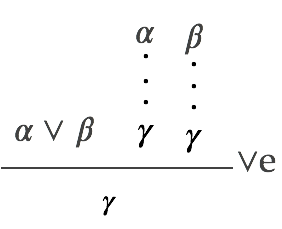
\includegraphics[scale=0.5]{orelim.png}
\caption{Disjunction-elimination ($\orelim$)}
\end{figure}

\begin{exercise}
Prove the following.
\begin{enumerate}
\item (commutative) $\alpha \vee \beta \proves \beta \vee \alpha$
\item (associative) $\alpha \vee (\beta \vee \gamma) \proves (\alpha \vee \beta) \vee \gamma$
\item (distributive) $\alpha \wedge (\beta \vee \gamma) \dashv \proves (\alpha \wedge \beta) \vee (\alpha \wedge \gamma)$.
\item $\alpha \vee (\beta \wedge \gamma) \dashv \proves (\alpha \vee \beta) \vee (\alpha \vee \gamma)$.
\end{enumerate}
\end{exercise}

\paragraph{False-elimination ($\falseelim$)} The rule says that, from a contradiction we can derive any formula. In other words, from falsity anything is provable. 
\begin{figure}[H]
\centering
\begin{prooftree}
\AxiomC{$\false$}
\RightLabel{\scriptsize $\falseelim$}
\UnaryInfC{$\alpha$}
\end{prooftree}
\caption{False-elimination ($\falseelim$)}
\end{figure}

\paragraph{Negation-elimination ($\negelim$)} Let us assume we are able to prove $\alpha$ and also prove $\neg \alpha$. Clearly we have proved a contradiction. The following rule can be used for proving contradictions.
\begin{figure}[H]
\centering
\begin{prooftree}
\AxiomC{$\alpha$}
\AxiomC{$\neg \alpha$}
\RightLabel{\scriptsize $\negelim$}
\BinaryInfC{$\false$}
\end{prooftree}
\caption{Negation-elimination ($\negelim$)}
\end{figure}

\paragraph{Negation-introduction ($\negintro$)} We are all used to proof by contradiction. This proof strategy assumes that a certain property is true and use that to prove a contradiction. This allow us to claim that our original assumption was wrong. This is exactly what this proof rule helps us to achieve.
\begin{figure}[H]
\centering
\begin{prooftree}
\alwaysNoLine
\AxiomC{$\alpha$}
\UnaryInfC{$.$}
\UnaryInfC{$.$}
\UnaryInfC{$.$}
\UnaryInfC{$\false$}
\alwaysSingleLine
\RightLabel{\scriptsize $\negintro$}
\UnaryInfC{$\neg \alpha$}
\end{prooftree}
\caption{Negation-introduction ($\negintro$)}
\end{figure}

Let us now some examples of natural deduction.

\begin{example}
Show that $\alpha \vee \beta, \alpha \vee \neg \beta \proves \alpha$.
\begin{figure}[H]
\centering
\begin{logicproof}{3}
  \alpha \vee \beta & axiom \\
  \alpha \vee \neg \beta & axiom \\
  \begin{subproof}
  \neg \alpha & assumption \\
  \begin{subproof}
	\begin{subproof}
		\alpha & assumption \\
  		\false & $\negelim$ 4,3 \\
  		\beta & $\falseelim$ 5
	\end{subproof}
	\begin{subproof}
  		\beta & assumption 
  	\end{subproof}
  		\beta & $\orelim$ 1, 4-6, 7
  	\end{subproof}
  	
  \begin{subproof}
   \begin{subproof}
		\alpha & assumption \\
  		\false & $\negelim$ 9,3 \\
  		\neg \beta & $\falseelim$ 10
  	\end{subproof}
	\begin{subproof}
  		\neg \beta & assumption 
  	\end{subproof}
  		\neg \beta & $\orelim$ 2, 9-11,12
  	\end{subproof}
  	\false & $\negelim$ 8,13
  	  	\end{subproof}
  	\neg \neg \alpha & $\negintro$ 3-14\\
  	\alpha & $\doublenegelim$ 15
\end{logicproof}
\caption{Proof of $\alpha \vee \beta, \alpha \vee \neg \beta \proves \alpha$}
\end{figure}
\end{example}

\begin{example}
Show that $\neg \alpha \proves \alpha \ifthen \beta$
\begin{figure}[H]
\centering
\begin{logicproof}{1}
	\neg \alpha & axiom \\
	\begin{subproof}
		\alpha & assumption \\
		\false & $\negelim$ 2, 1\\
		\beta & $\falseelim$ 3
	\end{subproof}
	\alpha \ifthen \beta & $\implintro$ 2-4
\end{logicproof}
\caption{Proof of $\neg \alpha \proves \alpha \ifthen \beta$}
\end{figure}
\label{example:negtoimpl}
\end{example}

\begin{example}
Show that $\neg \alpha \proves \neg (\alpha \wedge \beta)$
\begin{figure}[H]
\centering
\begin{logicproof}{1}
	\neg \alpha & axiom \\
	\begin{subproof}
		\alpha \wedge \beta & assumption \\
		\alpha & $\andelim{1}$ 2\\
		\false & $\negelim$ 3,1
	\end{subproof}
	\neg (\alpha \wedge \beta) & $\negintro$ 2-4
\end{logicproof}
\caption{Proof of  $\neg \alpha \proves \neg (\alpha \wedge \beta)$}
\end{figure}
\end{example}


\begin{exercise}[modus tollens] Show that $\alpha \ifthen \beta, \neg \beta \proves \neg \alpha$.
\label{exercise:modustollens}
\end{exercise}

\begin{exercise}[LEM]
Show that \true $~\proves \alpha \vee \neg \alpha$.
\label{exercise:lem}
\end{exercise}

\begin{figure}[H]
\centering
\includegraphics[width=1\textwidth]{allRules}
\caption{The rules of Natural Deduction}
\end{figure}


\section{Soundness theorem}
The proof of the theorem involves mathematical induction. If you are not used to induction, go through Chapter \ref{chap:mathInd}.

Let us restate the soundness theorem first.
\begin{theorem}[Soundness]
If $\Gamma \proves \psi$, then $\Gamma \models \psi$.
\label{thm:soundness}
\end{theorem}
The theorem says that, all formulas proved using natural deduction are true in a world where the axioms are true. The rest of this section will be devoted to proving the soundness theorem. The proof is by mathematical induction on the length of the proof. The length of a proof is the number of steps required in a natural deduction proof. The induction hypothesis is as follows:

\myquote{``For all set of formulas $\Gamma$, if $\Gamma \proves \psi$ where proof length is $n$, then $\Gamma \models \psi$ holds."}

Base Case ($n=1$): The only proof of length $1$ is as follows
\[
\Gamma \proves \alpha \text{~~--- Axiom}
\]
where $\alpha \in \Gamma$ is an axiom. From the definition of $\models$ it follows that $\Gamma \models \alpha$.

Inductive step: Let us assume that the induction hypothesis holds for all proofs of length less than or equal to $n$. We will show that the claim holds for proofs of length $n+1$. Consider one such proof. We will do a case analysis on the rule applied to derive $\psi$ in the $n+1$th step of the proof.

Case $\andintro$: The step is and-introduction. That is, we have $\Gamma \proves \psi$ and $\psi$ is of the form $\alpha \wedge \beta$ for some formulas $\alpha$ and $\beta$ which were derived earlier in the proof. Hence we know that $\Gamma \proves \alpha$ and $\Gamma \proves \beta$. From induction hypothesis (since the proof lengths are less than $n+1$) it follows $\Gamma \models \alpha$ and $\Gamma \models \beta$. From the semantics of $\wedge$, we get $\Gamma \models \alpha \wedge \beta$.

Case $\wedge e$: That means, $\Gamma \proves \psi$ and $\psi$ has been derived by applying an and elimination from a formula of the form $\psi \wedge \alpha$ or $\alpha \wedge \psi$. We will assume the former (the latter will have a symmetric argument). This means, there was a step in the proof which derived $\psi \wedge \alpha$ and hence $\Gamma \proves \psi \wedge \alpha$. Since the proof length of $\psi \wedge \alpha$ is less than $n+1$, from induction hypothesis we get $\Gamma \models \psi \wedge \alpha$. From the semantics of and ($\wedge$) it follows $\Gamma \models \psi$.

Case $\doublenegintro$: That is $\psi$ is of the form $\neg \neg \alpha$ for an $\alpha$ which was derived earlier in the proof. From induction hypothesis and semantics of negation (applied twice), it follows $\Gamma \models \psi$.

Case $\doublenegelim$: We can assume $\psi$ is got by elimination the double negation from a formula $\neg \neg \psi$ which was derived earlier in the proof. Again, applying induction hypothesis and using the semantics of negation, we get that $\Gamma \models \psi$.

Case $\implintro$: Let us assume that $\Gamma \proves \psi$ and $\psi$ is of the form $\alpha \ifthen \beta$ and the rule applied was implication-introduction. Therefore, after assuming $\alpha$, there is a derivation of $\beta$ in the proof. In other words, $\Gamma \cup \alpha \proves \beta$. This proof is of length less than $n+1$ and hence $\Gamma \cup \alpha \models \beta$. From the semantics of implication, it follows that $\Gamma \models \alpha \ifthen \beta$. 

Similarly going through all the other cases will finish the proof of the soundness theorem. The reader is asked to try showing this.

\begin{exercise}
Show the remaining cases, left out in Theorem \ref{thm:soundness}.
\end{exercise}

\section[Completeness: Huth \& Ryan]{Completeness theorem: Huth \& Ryan}
\label{sec:completeness}

We say that a formula $\alpha$ is a \indexit{theorem} if $\alpha$ can be proved without assuming any axioms. That is, $\true ~\proves \alpha$. 

In this section we prove the completeness theorem in a weaker setting, where $\Gamma$ is a finite set of formulas. The stronger result will be given later.
\begin{theorem}[Completeness]
\label{thm:completeness}
Let $\Gamma$ be a finite set of formulas. Then,  $\Gamma \models \psi$ implies $\Gamma \proves \psi$.
\end{theorem}
The theorem says that, if our formula is true in a world where the axioms are true, then the formula can be proved from the axioms. The rest of the section is proving the theorem. The proof strategy we follow is given in Figure \ref{fig:completenessHR}.

\begin{figure}[!h]
\centering
\begin{tikzpicture}[node distance = 0.75cm, auto]
    % Place nodes
    \node [block] (one) {1. Reduce completeness theorem to proving ``If $\alpha$ is a tautology then $\alpha$ is a theorem''.};
    \node [block, below of=one] (two) {2. For every valuation $v$, we give a formula $\beta_v$ and a proof  $\beta_v \proves \alpha$};
    \node [block, below of=two] (three) {3. We combine all the proofs above to show $\alpha$ is a theorem.};

    % Draw edges
    \path [line] (one) --node {} (two);
    \path [line] (two) --node {} (three);
    
\end{tikzpicture}
\caption{Proof of Completeness Theorem}
\label{fig:completenessHR}
\end{figure}

Our first step is to reduce the completeness theorem to a simpler case. 
\begin{lemma}
\label{lem:complete}
If $\alpha$ is a tautology, then $\alpha$ is a theorem. That is, if \true $~\models \alpha$, then \true $~\proves \alpha$
\end{lemma}

Before we prove the lemma, let us show how it would imply completeness theorem. Let us assume that $\Gamma = \{\alpha_1,\dots,\alpha_n\}$ and $\alpha_1,\alpha_2,\dots, \alpha_n \models \psi$.  From Exercise \ref{exercise:semequiv} we know this is equivalent to \true $~\models (\alpha_1 \wedge \alpha_2 \wedge \dots \alpha_n) \ifthen \psi$. Our Lemma \ref{lem:complete} shows that this is equivalent to \true $~\proves (\alpha_1 \wedge \alpha_2 \wedge \dots \alpha_n) \ifthen \psi$. From Exercise \ref{exercise:natequiv} it follows that $\alpha_1,\alpha_2,\dots,\alpha_n \proves \psi$. This finishes the completeness theorem.

Now we can go the proof of Lemma \ref{lem:complete}.
\begin{proof} [Proof of Lemma \ref{lem:complete}]
Let $P$ be the set of all propositions in $\alpha$. For a particular valuation, $v$ of $P$, we can define the following formula $\beta_v$ 
\[
\beta_v = \bigwedge_{\substack{p \in P \\ v(p) = \true}} p ~\wedge \bigwedge_{\substack{p \in P \\ v(p) = \false}} \neg p
\]
That is $\beta_v$ is the conjunction of all propositions which are assigned true in the valuation along with the neg of all propositions which are assigned false. Let $\alpha$ be an arbitrary formula. Then the following claim holds for any valuation $v$ because $\beta_v$ is satisfied by exactly one valuation, namely $v$. 
\begin{claim}
\[\beta_v \nmodels \alpha \mbox{ iff } \beta_v \models \neg \alpha\]
\end{claim}
See exercise \ref{exercise_uniqueval} for the proof of the above claim. We now prove the following for all subformulas $\psi$ of $\alpha$.
\begin{align}
\text{If } \beta_v \models \psi \text{ then } \beta_v \proves \psi \nonumber \\
\text{If } \beta_v \not \models \psi \text{ then } \beta_v \proves \neg \psi 
\label{align:induction}
\end{align}
The proof is by structural induction on the parse tree of $\alpha$. Let us do a case analysis of the type of node.

Case $\psi := p$: Let us first consider the case $\beta_v \models p$. Since $p$ is a conjunct in $\beta_v$ and-elimination gives us $\beta_v \proves p$. Now if $\beta_v \not \models p$, then $\beta_v \models \neg p$, which implies $\neg p$ is a conjunct in $\beta_v$. Therefore, $\beta_v \proves \neg p$.

Case $\psi := \gamma_1 \wedge \gamma_2$: Let us first consider the case $\beta_v \models \gamma_1 \wedge \gamma_2$. 
\begin{align*}
\text{Let } & \beta_v \models \gamma_1 \wedge \gamma_2 
\\ \implies & \beta_v \models \gamma_1 \text{ and } \beta_v \models \gamma_2  \tag{ semantics of and}
\\ \implies & \beta_v \proves \gamma_1 \text { and } \beta_v \proves \gamma_2  \tag{ induction hypothesis}
\\ \implies & \beta_v \proves \gamma_1 \wedge \gamma_2  \tag{ and-introduction}	
\end{align*}
Now let us prove the other if condition.
\begin{align*}
\text{Let } & \beta_v \nmodels (\gamma_1 \wedge \gamma_2) 
\\ \implies & \beta_v \models \neg (\gamma_1 \wedge \gamma_2) \tag{ definition of semantic entailment}
\\ \implies & \beta_v \models \neg \gamma_1 \vee \neg \gamma_2 \tag { Demorgan's law (proof in Exercise \ref{exercise:demorgansem})}
\\ \implies & \beta_v \nmodels  \gamma_1 \text{ or } \beta_v \nmodels  \gamma_2 \tag { semantics of or}
\\ \implies & \beta_v \proves \neg \gamma_1 \text { or } \beta_v \proves \neg \gamma_2 \tag { induction hypothesis}
\\ \implies & \beta_v \proves \neg \gamma_1 \vee \neg \gamma_2 \tag { or-introduction }
\\ \implies & \beta_v \proves \neg (\gamma_1 \wedge \gamma_2) \tag{ See Exercise \ref{exercise:demorgan} for this derivation}
\end{align*}

We have shown both sides of equation \ref{align:induction}. 

Case $\psi := \gamma_1 \vee \gamma_2$:  Let us first consider the case $\beta_v \models \gamma_1 \vee \gamma_2$. From the semantics of disjunction, it follows that $\beta_v \models \gamma_1$ or $\beta_v \models \gamma_2$. By induction hypothesis, we have $\beta_v \proves \gamma_1$ or $\beta_v \proves \gamma_2$. From or-introduction, it follows that $\beta_v \proves \gamma_1\vee\gamma_2$. Now let us assume $\beta_v \not \models \gamma_1 \vee \gamma_2$. From the semantics of disjunction and negation, it follows that $\beta_v \models \neg \gamma_1$ and $\beta_v  \models \neg \gamma_2$. By induction hypothesis, we have $\beta_v \proves \neg \gamma_1$ and $\beta_v  \proves \neg \gamma_2$. Now exercise \ref{exercise:demorgan} gives us $\beta_v \proves \neg (\gamma_1\vee \gamma_2)$.

Case $\psi := \neg \gamma$: Let us first assume $\beta_v \models \neg \gamma$. Therefore $\beta_v \nmodels \gamma$. From induction hypothesis, therefore it follows that $\beta_v \proves \neg \gamma$. Now, let us assume $\beta_v \nmodels \neg \gamma$. This is equivalent to $\beta_v \models \gamma$ which from induction hypothesis gives us $\beta_v \proves \gamma$. Introducing double negation will give us $\beta_v \models \neg \neg \gamma$.

Case $\psi := \gamma_1 \ifthen \gamma_2$: Let us consider the case $\beta_v \models \gamma_1 \ifthen \gamma_2$.
\begin{align*}
\text{Let } & \beta_v \models \gamma_1 \ifthen \gamma_2
\\ \implies & \beta_v \models \neg \gamma_1 \vee \gamma_2 \tag{ see Exercise \ref{exercise:implequiv}}
\\ \implies & \beta_v \nmodels \gamma_1 \text{ or } \beta_v \models \gamma_2  \tag{ semantics of or and negation}
\\ \implies & \beta_v \proves \neg \gamma_1 \text { or } \beta_v \proves \gamma_2  \tag{ induction hypothesis}
\\ \implies & \beta_v \proves \neg \gamma_1 \vee \gamma_2  \tag{ or-introduction}	
\\ \implies & \beta_v \proves \gamma_1 \ifthen \gamma_2 \tag{ see Exercise \ref{exercise:toimpl}}
\end{align*}

Now let us assume $\beta_v \not \models \gamma_1 \ifthen \gamma_2$. 
\begin{align*}
\text{Let } & \beta_v \nmodels \gamma_1 \ifthen \gamma_2
\\ \implies & \beta_v \models \neg (\neg \gamma_1 \vee \gamma_2) \tag{ see Exercise \ref{exercise:implequiv}}
\\ \implies & \beta_v \models \gamma_1 \text{ and } \beta_v \nmodels \gamma_2  \tag{ semantics of or and negation, demorgan}
\\ \implies & \beta_v \proves  \gamma_1 \text { and } \beta_v \proves \neg \gamma_2  \tag{ induction hypothesis}
\\ \implies & \beta_v \proves  \gamma_1 \wedge \neg \gamma_2  \tag{ and-introduction}	
\\ \implies & \beta_v \proves \neg (\gamma_1 \ifthen \gamma_2) \tag{ see Exercise \ref{exercise:toimpl}}
\end{align*}
Thus equation \ref{align:induction} is true for the implication case.

We have exhausted all the ways in which formulas can be built. Therefore, the claim in equation \ref{align:induction} holds. Let us go back to the lemma and assume its hypothesis,  $\true ~\models \alpha$. That is, for all valuations $v$ over the propositions, $\beta_v \models \alpha$. From our discussion above we have $\beta_v \proves \alpha$. Exercise \ref{exercise:theorem} now gives us $\true ~\proves \alpha$.
\end{proof}


\section[Completeness: Hintikka*]{Completeness: Alternate proof using Hintikka sets*}
In this section we give an alternate proof for completeness. We prove the simpler version, namely

\noindent {\bf Lemma \ref{lem:complete}.} \emph{If \true $~\models \alpha$, then \true $~\proves \alpha$}

As seen in the previous section, the above lemma along with the exercises \ref{exercise:semequiv} and \ref{exercise:natequiv}, will give us the completeness theorem. The rest of the section is for proving the above lemma.

Natural deduction gives us rules to derive proofs of statements. What is an important property these rules should satisfy? It should not help us to derive both a property and its negation. That is, we do not want natural deduction to satisfy $\true \proves \alpha$ and $\true \proves \neg \alpha$ for any formula $\alpha$. In fact if it does, then using natural deduction you can prove any formula. 
\begin{exercise}
If $\true \proves \alpha$ and $\true \proves \neg \alpha$, then $\true \proves \beta$ for all $\beta$.
\end{exercise}
So what we are interested in is a property called \indexit{consistency}. We say that a formula $\alpha$ is \indexit{consistent} if $\true ~\nproves \neg \alpha$. That is, $\alpha$ is consistent if there is no proof for $\neg \alpha$. Note that, this does not say that there is a proof for $\alpha$. The following theorem connects consistent formulas and Lemma \ref{lem:complete}. In fact, it also shows that natural deduction is consistent.
\begin{claim}
The following statements are equivalent.
\begin{enumerate}
\item If \true $~\models \alpha$, then \true $~\proves \alpha$
\item If $\neg \alpha$ is consistent, then $\neg \alpha$ is satisfiable.
\end{enumerate}
\end{claim}
\begin{proof}
$(1 \implies 2):$ Let $\neg \alpha$ be consistent. That is  \true $~\nproves \neg \neg \alpha$.
Therefore \true $~\nproves \alpha$ (otherwise contradiction by double-negation introduction). From $(1)$ we get \true $~ \nmodels \alpha$ and hence $\neg \alpha$ is satisfiable.

\noindent $(2 \implies 1):$ Let \true $~\models \alpha$. Therefore $\neg \alpha$ is not satisfiable. From $(2)$ we get $\neg \alpha$ is not consistent. In other words \true $~\proves \neg \neg \alpha$. The claim now follows from double-negation elimination.
\end{proof}
We will now prove that ``If $\beta$ is consistent, then $\beta$ is satisfiable". For a finite set $X$ of formulas, we say $X$ is consistent if the formula $\bigwedge_{\alpha \in X} \alpha$ is consistent. Given a consistent set $X$, we can extend the sets in a meaningful way as follows. Let us order all propositional logic formulas into a sequence
 \[\alpha_0,\alpha_1,\dots\]
We define $X_0 = X$ and for all $i \geq 0$ we define $X_{i+1}$ as follows.
\[
X_{i+1} = \begin{cases}
X_i \text{, if } X_i \cup \alpha_i \text{ is not consistent } \\
X_i \cup \alpha_i \text{, otherwise}
\end{cases}
\]

We now define the maximal consistent extension of $X$, (denoted by $\hat X$) as $\bigcup_{i \geq 0} X_i$. This maximal consistent set satisfy some interesting properties.
\begin{lemma}
Let $\hat X$ be as defined above. Then
\begin{enumerate}
\item For all  $i \geq 0$, $\alpha_i \in \hat X$ iff $\neg \alpha_i \notin \hat X$. 
\item For all  $i,j \geq 0$, $\alpha_i \wedge \alpha_j \in \hat X$ iff $\alpha_i \in \hat X$ and $\alpha_j \in \hat X$.
\item For all  $i,j \geq 0$, $\alpha_i \vee \alpha_j \in \hat X$ iff $\alpha_i \in \hat X$ or $\alpha_j \in \hat X$.
\item For all  $i,j \geq 0$, $\alpha_i \ifthen \alpha_j \in \hat X$ iff $\alpha_i \notin \hat X$ or $\alpha_j \in \hat X$.
\end{enumerate}
\label{lem:mcs}
\end{lemma}
\begin{proof}
We will prove each of the above claims.
\begin{enumerate}
\item Let $\alpha_j = \neg \alpha_i$ and $k = max \{i,j\}$. We show that  $\alpha_i \in X_k$ iff $\alpha_j \notin X_k$. Let $\beta = \bigwedge_{i=0}^k \alpha_i$. Let us first assume that both $\alpha_i$ and $\neg \alpha_i$ are not in $X_k$. Then, $\beta \wedge \alpha_i$ and $\beta \wedge \neg \alpha_i$ are not consistent. Therefore \true $~\proves \neg (\beta \wedge \alpha_i)$ and \true $~\proves \neg (\beta \wedge \neg \alpha_i)$. From Example \ref{example:negtoimpl}, it follows that \true $~\proves \neg \beta$. This is a contradiction, since $\beta$ is consistent. Now, let us assume both $\alpha_i$ and $\neg \alpha_i$ both are in $X_k$. That is, \true $~ \nproves \neg (\beta \wedge \alpha_i \wedge \neg \alpha_i)$. This is a contradiction from exercise \ref{exercise:lem}. Therefore either one of $\alpha_i$ or $\alpha_j$ should be in $X_k$ and hence in $\hat X$.
\item Let $\alpha_l = \alpha_i \wedge \alpha_j$ and $k = max\{i,j,l\}$. We show that  $\alpha_l \in X_k$ iff $\alpha_i \in X_k$ and $\alpha_j \in X_k$. Let $\beta = \bigwedge_{i=0}^k \alpha_i$. First, let us assume $\alpha_l \notin X_k$. That is, \true $~\proves \neg (\beta \wedge \alpha_i \wedge \alpha_j)$. From Demorgan's exercise \ref{exercise:demorgan} we know this is equivalent to \true $~\proves \neg \beta \vee \neg \alpha_i \vee  \neg \alpha_j$. Since $\beta$ is consistent, \true $~\nproves \neg \beta$. Therefore (semantics of disjunction) gives, \true $~\proves  \neg \alpha_i$ or \true $~\proves  \neg \alpha_j$. This shows that either $\alpha_i \notin X_k$ or $\alpha_j \notin X_k$. Now let us consider the other direction of the claim. Let $\alpha_i \notin X_k$ or $\alpha_j \notin X_k$. In other words, \true $~\proves  \neg \alpha_i$ or \true $~\proves  \neg \alpha_j$. Applying or-introduction and demorgan's laws we get \true $~\proves \neg (\beta \wedge \alpha_i \wedge \alpha_j)$. Therefore $\alpha \in X_k$. This proves the forward direction of the claim.
\end{enumerate}

We leave the rest of the claims for the reader to prove.
\end{proof}

\begin{exercise}
Prove the remaining cases in Lemma \ref{lem:mcs}.
\end{exercise}

Our next lemma says that if a formula $\beta$ is in $\hat X$, then $\beta$ is satisfiable. 
\begin{lemma}
If $\beta \in \hat X$, then $\beta$ is satisfiable.
\label{lem:consistimplsat}
\end{lemma}
\begin{proof}
Let $V$ be a set which contains either propositions or its negations. We define $V$ as follows. If $p \in \hat X$, then $p \in V$. On the other hand, if $p \notin \hat X$, then $\neg p \in V$. It is easy to see that, there is a satisfying assignment which makes all formulas in $V$ true. We are done, if we show that $V \models \beta$. We prove the following induction hypothesis by structural induction on subformulas of $\beta$.
\[
\gamma \in \hat X \iff V \models \gamma
\]

Case $\gamma=p$, a proposition: If $p \in \hat X$, by definition $V \models \gamma$. On the other hand, if $p \notin \hat X$, we have by definition $V \models \neg p$ and therefore $V \nmodels p$.

Case $\gamma = \neg \psi$: If $\neg \psi \in \hat X$, then (by properties of $\hat X$, Lemma \ref{lem:mcs}) $\psi \notin \hat X$. By our induction hypothesis it follows $V \nmodels \psi$ and therefore (semantics of negation) $V \models \neg \psi$. Let us assume $\neg \psi \notin \hat X$. By Lemma \ref{lem:mcs}, $\psi \in \hat X$, which by IH gives us $V \models \psi$. Therefore $V \nmodels \neg \psi$.

Case $\gamma = \psi_1 \wedge \psi_2$: If $\psi_1 \wedge \psi_2 \in \hat X$, then (Lemma \ref{lem:mcs}) $\psi_1 \in \hat X$ and $\psi_2 \in \hat X$. By IH, $V \models \psi_1$ and $V \models \psi_2$ and therefore $V \models \psi_1 \wedge \psi_2$. Let us now assume $\psi_1 \wedge \psi_2 \notin \hat X$. Therefore (Lemma \ref{lem:mcs}) $\psi_1 \notin \hat X$ or $\psi_2 \notin \hat X$. From IH, we get $V \nmodels \psi_1$ or $V \nmodels \psi_2$. Therefore $V \models \neg \psi_1 \vee \neg \psi_2$. Which by demorgan's laws proves the case.

We leave the rest of the case as exercise.
\end{proof}
\begin{exercise}
Prove the remaining cases in Lemma \ref{lem:consistimplsat}.
\end{exercise}

We now have enough understanding to prove the completeness theorem. \\

\noindent {\bf Proof of Lemma \ref{lem:complete}.} Let $\neg \alpha$ be consistent. Extend the set $X = \{\neg \alpha\}$ to $\hat X$, the maximal consistent set. Lemma \ref{lem:consistimplsat}, gives that all formulas in $\hat X$ are satisfiable and therefore $\neg \alpha$ is satisfiable too. \qed

\section{Strong Completeness*}
In Section \ref{sec:completeness} we saw the completeness theorem for the case when $\Gamma$ is finite. In this section we will show that the completeness theorem is true even for the infinite case. Compactness theorem will help us in this regard.

\begin{theorem}[Strong completeness]
Let $\Gamma$ be a set of formulas and $\psi$ be a formula. Then $\Gamma \proves \psi$ if $\Gamma \models \psi$.
\end{theorem}
\begin{proof}
Let $\Gamma \models \psi$. Therefore $\Gamma \nmodels \neg \psi$. It follows that $\Gamma \cup \neg \psi$ is not satisfiable. The compactness theorem of propositional logic (Theorem \ref{thm:propCompactness}) gives us that there exists a finite subset $\Gamma' \subseteq \Gamma$ such that $\Gamma' \cup \neg \psi$ is not satisfiable. Therefore we have $\Gamma' \nmodels \neg \psi$. In other words $\Gamma' \models \psi$. From the completeness theorem for propositional logic (see Theorem \ref{thm:completeness}) we have $\Gamma' \proves \psi$. Since $\Gamma' \subseteq \Gamma$, we have $\Gamma \proves \psi$.
\end{proof}

\section{Exercises}
\begin{exercise}[syntactic variant of De Morgan's law]
Prove the following.
\begin{multicols}{2}
\begin{enumerate}
\item $\neg (\alpha \wedge \beta) \dashv \proves \neg \alpha \vee \neg \beta$
\item $ \neg \alpha \wedge \neg \beta \dashv \proves  \neg (\alpha \vee \beta)$
\end{enumerate}
\end{multicols}
\label{exercise:demorgan}
\end{exercise}

\begin{exercise}[Hilbert's axioms]
Prove the following.
\begin{multicols}{2}
\begin{enumerate}
\item \true $~ \vdash \big(\alpha \ifthen (\beta \ifthen \alpha)\big)$
\item \true $~ \vdash \big(\neg \beta \ifthen \neg \alpha \big) \ifthen \big(\alpha \ifthen \beta \big)$
\end{enumerate}
\end{multicols}
\begin{enumerate} 
\item [3.] \true $~ \vdash \big(\alpha \ifthen (\beta \ifthen \gamma)\big) \ifthen \big((\alpha \ifthen \beta) \ifthen (\alpha \ifthen \gamma)\big)$
\end{enumerate}
\end{exercise}

\begin{exercise}
Show that the following are equivalent
\begin{multicols}{2}
\begin{enumerate}
\item $\alpha_1, \alpha_2, \dots, \alpha_n \proves \beta$
\item \true $~\proves (\alpha_1 \wedge \alpha_2 \wedge \dots \alpha_n) \ifthen \beta$
\end{enumerate}
\end{multicols}
\begin{enumerate}
\item [3.] \true $~\proves \Big(\alpha_1 \ifthen \big(\alpha_2 \ifthen (\dots (\alpha_n \ifthen \beta))\big)\Big)$
\end{enumerate}
\label{exercise:natequiv}
\end{exercise}

\begin{exercise}
Prove the following.
\begin{multicols}{2}
\begin{enumerate}
\item $\neg \gamma_1 \vee \gamma_2  \dashv \proves \gamma_1 \ifthen \gamma_2$ 
\item $\gamma_1 \wedge \neg \gamma_2  \dashv \proves \neg (\gamma_1 \ifthen \gamma_2)$	 
\item $\neg \alpha \proves \alpha \ifthen \beta$
\item $\alpha \ifthen \beta, \beta \ifthen \alpha \proves \alpha \ifthen \gamma$
\end{enumerate}
\end{multicols}
\label{exercise:toimpl}
\end{exercise}

\begin{exercise}
Show that the following are theorems
\begin{multicols}{2}
\begin{enumerate}
\item $\alpha \vee \neg \alpha$
\item $\alpha \ifthen \alpha$
\item $\alpha \ifthen \neg \neg \alpha$
\item $(\alpha \ifthen \beta) \ifthen (\neg \beta \ifthen \neg \alpha)$
\item $(\neg \alpha \ifthen \alpha) \ifthen \alpha$
\item $ (\neg \alpha \ifthen (\alpha \ifthen \beta))$
\item $ \neg \neg \alpha \ifthen \alpha$
\item $(\alpha \ifthen \beta) \ifthen ((\alpha \ifthen \neg \beta) \ifthen \neg \beta))$
\end{enumerate}
\end{multicols}
\end{exercise}



\begin{exercise}
Let $\Psi$ be a formula over only the proposition $p$. Assume that $p \proves \psi$ and $\neg p \proves \psi$. Show that,  \true $~\proves \psi$.
\end{exercise}

\begin{exercise}
 Let us introduce a new connective xor: $\alpha \xor \beta$ which should abbreviate $(\neg \alpha \wedge \beta) \vee (\alpha \wedge \neg \beta)$. Design introduction and elimination rules for xor.
\end{exercise}

\begin{exercise}
Let $P = \{p_1,\dots,p_n\}$ be a set of propositions. For a valuation $v$ over $P$, we define $\Gamma_v = \{p_i ~|~ v(p_i) = \true \} \cup \{\neg p_i ~|~ v(p_i) = \false \}$. Consider a formula $\alpha$ such that $\Gamma_v \proves \alpha$ for all valuation $v$. Show that $\true ~\proves \alpha$.
\label{exercise:theorem}
\end{exercise}

\begin{exercise}
\label{exercise_uniqueval}
Let $v$ be a valuation. Then the following holds for all formulas $\alpha$.
\[
\beta_v \nmodels \alpha \mbox{ iff } \beta_v \models \neg \alpha
\]
\end{exercise}

\begin{exercise}
[Strong soundness theorem] If $\Gamma \proves \alpha$ then $\Gamma \models \alpha$.
\end{exercise}
\begin{exercise}
If $\Gamma$ is satisfiable then $\Gamma$ is consistent.
\end{exercise}

\begin{exercise}
Consider a new natural deduction set of rules you have created. Let $\Gamma$ be a set of propositional formulas (the set need not be finite). Let us also define by $\Gamma \proves^* \alpha$ to be a proof of $\alpha$ from $\Gamma$ using your natural deduction rules. Let us also say that $\Gamma$ is consistent, if you cannot prove $\alpha$ or $\neg \alpha$ using your natural deduction rules for any $\alpha$ from $\Gamma$. Prove that the following two statements are equivalent.
\begin{enumerate}
\item If $\Gamma \proves^* \alpha$ then $\Gamma \models \alpha$.
\item If $\Gamma$ is satisfiable then $\Gamma$ is consistent.
\end{enumerate}
\end{exercise}

\begin{exercise}
Design introduction and elimination rules for Nand operator. Consider the logic which uses only negation and Nand operator as logical symbols. Prove the completeness theorem using the introduction and elimination rules for Nand and negation. Prove also the soundness theorem.
\end{exercise}
 
\begin{exercise}
Prove the deduction theorem for a set (need not be finite) $\Gamma$ of propositional formulas : $\Gamma \proves (\alpha \ifthen \beta)$ iff $\Gamma \cup \{\alpha\} \proves \beta$.
\end{exercise}

\begin{exercise}
Prove or disprove the following statements.
\begin{enumerate}
\item If $\Gamma_1 \subseteq \Gamma_2$ and $\Gamma_1$ is consistent then $\Gamma_2$ is consistent.
\item If $\Gamma_1 \subseteq \Gamma_2$ and $\Gamma_2$ is consistent, then $\Gamma_1$ is consistent.
\end{enumerate}
\end{exercise}
%\chapter{Resolution}
\input{satSolvers.tex}
\newcommand{\expectation}[1]{E[#1]}
\newcommand{\prb}[1]{\mathtt{Prob}~[#1]}

\chapter{Randomized SAT Solvers}
In this chapter we will look at randomized algorithms for propositional formulas. In the first section, we give a polynomial time algorithm for checking satisfiability for 2-CNF formulas. Then we give an exponential time algorithm checking satisfiability for 3-CNF formulas. This algorithm will be better than the trivial $O(2^n)$ algorithm of going through all the assignments to the $n$ propositions. You will observe that both the algorithms are easy to describe. The difficult part is proving that the algorithm answers correctly with ``high" probability. 

\section{$2$-CNF}
The algorithm is given in Algorithm \ref{alg:randtwocnf}. In the algorithm the number of times the loop needs to be iterated (i.e. $m$) will be fixed later depending on the confidence in the algorithm the user requires.

\begin{algorithm}
 \caption{$2$-CNF Satisfiability}
 \label{alg:randtwocnf}
 \begin{algorithmic}[1]
 \renewcommand{\algorithmicrequire}{\textbf{Input:}}
 \renewcommand{\algorithmicensure}{\textbf{Output:}}
 \REQUIRE A $2$-CNF formula $\alpha$
 \ENSURE  $\alpha$ is satisfiable or not.
 \STATE Start with an arbitrary truth assignment.
 \FOR {$m$ steps} 
 \IF {assignment makes $\alpha$ true}
 \STATE Return SAT
 \ENDIF
 \STATE Choose a clause not satisfiable.
 \STATE Choose uniformly at random one of the propositions in the clause and change its assignment.
 \ENDFOR
 \STATE Return UNSAT.
 \end{algorithmic} 
 \end{algorithm}
 
The following claim is an easy observation about the algorithm. 
\begin{lemma}
If the formula $\alpha$ is unsatisfiable then Algorithm \ref{alg:randtwocnf} returns UNSAT. Contra positively, if the algorithm returns SAT, then the formula is satisfiable.
\end{lemma}

Due to the above lemma, the important question we need to answer is, if the formula is satisfiable, how often will the algorithm return UNSAT. That is, what is the probability that the algorithm fails. So, let us assume that the formula is satisfiable and try to answer how long will the algorithm take to return SAT. This will help us in deciding what is a good value for $m$.  

We now try to estimate the expected running time of the algorithm, assuming the formula is satisfiable and the loop runs for ever (i.e $m= \infty$). Let $S$ be a satisfying assignment for $\alpha$. We will try to find the expected running time for finding $S$. Note that, there may be other satisfying assignments and the algorithm might find them before it finds $S$. Therefore, the expected running time we find is a worst case estimate. Consider the $i^{th}$ iteration of the loop. We define $A_i$ and $X_i$ as follows
\[
A_i = \text{ the assignment at the beginning of the }i^{th} \text{ iteration of the loop} 
\]
\[
X_i = \text{ the number of variables whose assignments in } A_i \text{ differ from that of }S
\]

We can try to understand some properties of $X_i$. Note that if $X_i = n$, then all assignments to variables in $A_i$ differ from $S$. The algorithm therefore will find a clause which is not satisfiable. In that clause, assignments to both the propositions are wrong and hence no matter which proposition we pick and change the assignment we get that $X_{i+1}=n-1$.
\[
\prb{X_{i+1} = n-1 ~|~ X_i = n} = 1
\]
Let us now move on to the general case when $X_i = k<n$. We are interested in identifying the probability of $X_{i+1} = k-1$. Let us analyse our algorithm. We have $k$ assignments differing from $S$ and our algorithm picks a clause which is not satisfiable. Atleast one of the proposition in this clause is assigned a truth value in $A_i$ which is different from that in $S$ (note that, it could happen that both the propositions are assigned differently). Our algorithm picks one of the two proposition with equal probability and changes its assignment. Therefore, we pick a proposition whose value is different with probability greater than or equal to $\frac{1}{2}$. If both the propositional values are different we pick with probability $1$. Otherwise we pick with probability $\frac{1}{2}$. Therefore
\[
\prb{X_{i+1} = k-1 ~|~ X_i = k} \geq \frac{1}{2}
\]
A similar analysis also gives us
\[
\prb{X_{i+1} = k+1 ~|~ X_i = k} \leq \frac{1}{2}
\]

Our current understanding is captured by the following set of equations and in Figure \ref{fig:twocnfwalk}.
\begin{equation}
\label{eq:twoexactcnf}
\begin{split}
\prb{X_{i+1} = n-1 ~|~ X_i = n} = 1 \\
\prb{X_{i+1} = k-1 ~|~ X_i = k} \geq \frac{1}{2} ~, \forall k, \text{ where } 0< k < n\\
\prb{X_{i+1} = k+1 ~|~ X_i = k} \leq \frac{1}{2}~, \forall k, \text{ where } 0< k < n
\end{split}
\end{equation}
Let us assume that when we enter the first loop, we have an assignment such that $X_1 = k$. We are interested in finding out how many steps $m$ are required such that $X_m = 0$. Note that, at any iteration of the loop, we can go right one step in the figure (towards $n$) with probability greater than or equal to half and we can move left (towards $0$) with probability, less than or equal to half.

\begin{SCfigure}[1][h]
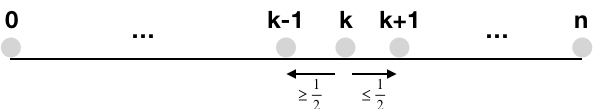
\includegraphics[width=0.5\textwidth]{twocnfwalk}
\caption{At each loop iteration, the algorithm walks one step towards the left or right with probability $\geq \frac{1}{2}$ or $\leq \frac{1}{2}$ respectively.}
\label{fig:twocnfwalk}
\end{SCfigure}

The walk given by Equation \ref{eq:twoexactcnf} is difficult to analyse and therefore we analyse a ``pessimistic" version of the above probability distribution. The equations in this version are approximated by a ``Markov chain" as follows (see also Figure \ref{fig:twoapproxcnfwalk}).
\begin{equation}
\label{eq:twocnf}
\begin{split}
\prb{X_{i+1} = n-1 ~|~ X_i = n} = 1 \\
\prb{X_{i+1} = k-1 ~|~ X_i = k} = \frac{1}{2} ~, \forall k, \text{ where } 0< k < n\\
\prb{X_{i+1} = k+1 ~|~ X_i = k} = \frac{1}{2}~, \forall k, \text{ where } 0< k < n
\end{split}
\end{equation}

\begin{SCfigure}[1][h]
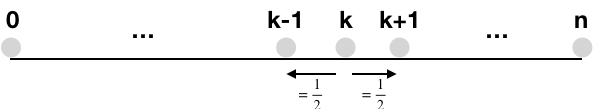
\includegraphics[width=0.5\textwidth]{twoapproxcnfwalk}
\caption{Markov Chain approximation: At each loop iteration, the algorithm walks one step towards the left or right with probability exactly $\frac{1}{2}$. This is a worst case scenario for our algorithm.}
\label{fig:twoapproxcnfwalk}
\end{SCfigure}

Note that, in the former setting, the probability of going left at any point was greater or equal to in the latter setting. Therefore, the probability of reaching $0$ in $m$ number of steps is greater in the former than in the latter. Therefore, the expected number of steps to reach $0$ from $k$ using these set of equations is greater than what we had before. We will give an upperbound for these sets of equations. 

Let $k$ be such that $0 \leq k \leq n$. We will denote by $Z_k$, the random variable representing the number of steps from $k$ to $0$. We are interested in the expected value of $Z_n$ (denoted by 
 $\expectation{Z_n}$). The Equations \ref{eq:twocnf} gives us the following
\begin{equation}
\label{eq:twocnfexpectation}
\begin{split}
\expectation{Z_0} = 0 \\
\expectation{Z_n} = 1 + \expectation{Z_{n-1}} \\
 \forall ~0<k<n, ~\expectation{Z_k} = \frac{1}{2} (1+\expectation{Z_{k-1}}) + \frac{1}{2}(1+\expectation{Z_{k+1})} \\
  = 1 + \frac{1}{2} (\expectation{Z_{k-1}} + \expectation{Z_{k+1}}) 
\end{split}
\end{equation} 

This contains $n+1$ equations on $n+1$ variables. The following claim holds for equations \ref{eq:twocnfexpectation}.
\begin{lemma}
For all $k$, where $0\leq k < n$ we have $\expectation{Z_k} = 2nk-k^2$
\end{lemma}
\begin{proof}
The proof is by induction on $k$. It is easy to observe that the claim holds for the base case $k=0$. Let us assume it true for some $k$ and show that it holds for $k+1$. We know the following
\[
\expectation{Z_k} = 1 + \frac{1}{2} (\expectation{Z_{k-1}} + \expectation{Z_{k+1}}) 
\]
Therefore, the lemma holds due to the following analysis
\begin{align*}
\expectation{Z_{k+1}} & = 2 \big(\expectation{Z_k} - 1 \big) - \expectation{Z_{k-1}} \\
& = 2 (2nk- k^2 -1 ) -  \big( 2n (k-1) - (k-1)^2 \big)  \\
& = 2 (2nk - k^2 -1 ) - \big( 2nk - 2n - (k^2 -2k + 1) \big) \\
& = 2nk - k^2 -1 + 2n - 2k \\
& = 2n(k+1) - (k+1)^2 
\end{align*}
\end{proof}

From this, we get that 
\[
\expectation{Z_n} = 1 + 2n (n-1) - (n-1)^2 = n^2
\]
In other words, the expected number of steps required from any position $k$ to $0$ is less than or equal to $n^2$. This proves the following.
\begin{lemma}
If a $2$-CNF formula is satisfiable, then the algorithm \ref{alg:randtwocnf} outputs SAT in an expected running time of at most $n^2$. 
\end{lemma}

With the above lemma, we can derive a ``good" value for $m$. We show that, if $m=2n^2t$, then the algorithm answers correctly with a probability greater than or equal to $(1 - \frac{1}{2^t})$. 
\begin{theorem}
Let $m = 2n^2t$. Then Algorithm \ref{alg:randtwocnf}. fails with probability less than or equal to $\frac{1}{2^t}$.
\end{theorem}
\begin{proof}
We know that if the formula is not satisfiable, the algorithm does not fail. So, let us assume that the formula is satisfiable. Let $Z$ be the random variable representing the number of steps taken to output SAT. Applying Markov's inequality to the above lemma gives us
\[
\prb{Z \geq 2n^2}  \leq \frac{1}{2}
\]
Let us consider our algorithm as running $t$ loops with each loop running $2n^2$ times. Then, an inside loop fails with probability less than or equal to half. Hence, the probability of the algorithm failing $t$ times is given by the union bound as 
\[
\prb{\text{ algorithm fails }} \leq \frac{1}{2^t}
\]


\end{proof}

\section{$3$-CNF}
Our algorithm will be a modification of the $2$-CNF algorithm. What could go wrong if we applied the same algorithm for the $3$-CNF case. The Markov chain for a $3$-CNF formula is given in Figure \ref{fig:threecnfwalk}. Exercise \ref{ex:threecnf} shows that the expected running time for this algorithm is $O(2^n)$. This is not good enough, since even going through all possible solutions takes only this much time. 

\begin{SCfigure}[1][h]
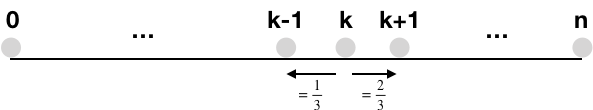
\includegraphics[width=0.5\textwidth]{threecnfwalk}
\caption{Markov Chain approximation: At each loop iteration, the algorithm walks one step towards the left or right with probability $\frac{1}{3}$, and $\frac{2}{3}$ respectively. This is a worst case scenario for our algorithm.}
\label{fig:threecnfwalk}
\end{SCfigure}

We modify our algorithm as follows.
\begin{algorithm}
 \caption{$3$-CNF Satisfiability}
 \label{alg:randthreecnf}
 \begin{algorithmic}[1]
 \renewcommand{\algorithmicrequire}{\textbf{Input:}}
 \renewcommand{\algorithmicensure}{\textbf{Output:}}
 \REQUIRE A $3$-CNF formula $\alpha$
 \ENSURE  $\alpha$ is satisfiable or not.
 \FOR {$m$ steps}
	 \STATE Start with an arbitrary truth assignment.
	 \FOR {$3n$ steps} 
		 \IF {assignment makes $\alpha$ true}
			 \STATE Return SAT
		 \ENDIF			 
		 \STATE Choose a clause not satisfiable.
		 \STATE Choose uniformly at random one of the propositions in the clause and change its assignment.
 	\ENDFOR
 \ENDFOR
 \STATE Return UNSAT.
\end{algorithmic} 
\end{algorithm}

As in the $2$-CNF algorithm, we know that if the formula is unsatisfiable, then the algorithm will return UNSAT. Let us now calculate the expected running time of the algorithm if $m=\infty$ and assuming the formula is satisfiable. Like in the previous analysis, let $S$ be the satisfying assignment. Let us now consider the run of an outer loop. We start from an arbitrary assignment for $\alpha$.  For the $i^{th}$ iteration of the inner loop we denote by $A_i$ the assignment at the beginning of the inner loop. We want to bound the probability that the $3n$ steps of the inner loop does not identify the satisfying assignment. Let us assume that the after the initial arbitrary assignment, $k$ many propositions are wrongly assigned. Let us denote by $q_k$ the probability that we reach a satisfying assignment within $3n$ steps of the inner loop. That is, the probability of reaching $0$ from $k$ by doing a random walk on the Markov Chain given in Figure \ref{fig:threecnfwalk}. Note that, in the special case of $k=0$, we have $q_0 = 1$. For a general $k>0$, there is no bound on the number of left or right moves required to reach $0$. Let us consider, a special case when the number of right moves is $k$ and the number of left moves is $2k$. Clearly $q_k$ is greater than the probability of this happening. Thus
\[
q_k \geq {3k \choose k} \big(\frac{1}{3}\big)^{2k} \big( \frac{2}{3} \big)^k
\]

Stirling's formula gives that there are constants $c_1$ and $c_2$ such that for any $n>0$, we have $c_1 \sqrt{n} \big(\frac{n}{e}\big)^n \leq n! \leq  c_2 \sqrt{n} \big(\frac{n}{e}\big)^n$. This can now be used to find a better bound for $q_k$.
\begin{align*}
q_k & \geq \frac{3k!}{k!}{2k!} \big(\frac{1}{3}\big)^{2k} \big( \frac{2}{3} \big)^k \\
& \geq \frac{c_1\sqrt{3k} (\frac{3k}{e})^{3k}}{c_2 \sqrt{k} (\frac{k}{e})^k c_2 \sqrt{2k} (\frac{2k}{e})^{2k}} \big(\frac{1}{3}\big)^{2k} \big( \frac{2}{3} \big)^k \\
& \geq c \frac{1}{\sqrt{k}} \frac{1}{2^k} \text{  , for a constant } c
\end{align*}

We now have a bound on $q_k$. Let us now calculate the probability $q$ that we find the satisfying assignment given that we start from a random assignment. Then,
\begin{align*}
q & = \sum_{k=0}^n \prb{\text{assignment to exactly $k$ propositions are different from that of } S ~} \times q_k \\
& \geq \frac{1}{2^n} + \sum_{k=1}^n {n \choose k} \frac{1}{2^n}  \frac{c}{\sqrt{k}} \frac{1}{2^k} \\
& \geq \frac{1}{2^n} \frac{c}{\sqrt{n}} + \sum_{k=1}^n {n \choose k} \frac{1}{2^n}  \frac{c}{\sqrt{n}} \frac{1}{2^k} \\
& = \frac{c}{\sqrt{n}2^n} \sum_{k=0}^n {n \choose k}  \frac{1}{2^k}  \\
& = \frac{c}{\sqrt{n}2^n} (1 + \frac{1}{2})^n ~(\text{ using the expansion for } (1 + \frac{1}{2})^n ) \\
& = \frac{c}{\sqrt{n}} \big(\frac{3}{4}\big)^n 
\end{align*}

Thus the probability of success starting from an arbitrary assignment and walking $3n$ steps is $\geq \frac{c}{\sqrt{n}} \big(\frac{3}{4}\big)^n$. Thus the expected running time of the outer loop for success is given by 
\[
O(\sqrt{n} \big(\frac{4}{3}\big)^n)
\]
Let $a$ be denoted by this number. Thus the total number of steps of the algorithm is $a \times 3n$. We will now show that taking $m = 2at$ will ensure that the probability of failure of our algorithm is less than or equal to $\frac{1}{2^t}$. 
\begin{theorem}
Let $a = \frac{\sqrt{n}}{c} \big(\frac{4}{3}\big)^n)$ and $m = 2at$. Then the running time of Algorithm \ref{alg:randthreecnf}. is $O(n^{\frac{3}{2}}\big(\frac{4}{3}\big)^n)$ and the probability of failure is less than or equal to $\frac{1}{2^t}$. 
\end{theorem}
\begin{proof}
The running time of the algorithm is $3n \times \frac{\sqrt{n}}{c} \big(\frac{4}{3}\big)^n) = O(n^{\frac{3}{2}}\big(\frac{4}{3}\big)^n)$. The algorithm will fail only if the formula is satisfiable. Let $Z$ be the random variable denoting the number of outer loops required for finding the satisfying assignments. Using Markov's inequality we can show that
\[
\prb{Z \geq 2a} \leq \frac{1}{2}
\]
Let us again consider that we are running the algorithm $t$ times and each time we are running the outer loop for $2a$ times. Thus the probability of failure for all the $t$ times is given by the union bound by
\[
\prb {\text{algorithm fails }} \leq \frac{1}{2^t}
\]

\end{proof}



%\section{Randomized solvers}
%\subsection{2 CNF: Randomized polynomial time}
%\subsection{3 CNF}
%\chapter{SAT Counting}
%\section{CNF counting}
%\subsection{\# P-complete}
%\subsection{Randomized approximate counting}
%\section{DNF counting: FPRAS algorithm}
%\chapter{Max-SAT}
%\section{PCP: Hardness of approximation}

\part{First Order Logic}
\chapter{First Order Logic}
\section{Introduction}
Consider the logical derivations in Table \ref{tab:ramaujanProofs}. Which one of the reasoning is correct?

\begin{table}[H]
\centering
\begin{tabular}{p{74mm}|p{82mm}}
%\hline
Proof A \newline
1. All mathematicians are intelligent.\newline
2. Ramanujan was a mathematician.\newline
3. Therefore, Ramanujan was intelligent. &
Proof B \newline
1. There is a mathematician who is intelligent. \newline
2. Ramanujan was a mathematician. \newline
3. Therefore, Ramanujan was intelligent. \\
%\hline
\end{tabular}
\caption{Two proofs - One is correct, one wrong.}
\label{tab:ramaujanProofs}
\end{table}

You could see that Proof A is correct, whereas Proof B is not. Natural deduction of propositional logic will not help us to reach a correct conclusion. We need a stronger, richer logic for these kind of reasoning. We will show that, \indexit{first order logic} (also called \indexit{predicate} logic) will help us. 

Consider the following statement. 
\begin{equation}
\text{Everyone is younger than a father.}
\label{eq:fostatement}
\end{equation}
Our aim is to capture the information contained in the statement. We first introduce a \indexit{predicate} called father (which will be denoted by $F$). Introducing this predicate, allows us to write a formula like 
\[F(Ashoka)\]
The meaning we intend to convey is, ``Ashoka is a father". We can thus write $F(Alexander), F(Shivaji)$ etc. Let us introduce another predicate younger (which will be denoted by $Y$). We denote by $Y(Shivaji, Ashoka)$ to mean ``Shivaji is younger than Ashoka". The difference between the predicates $F$ and $Y$ is that $F$ takes one value as parameter whereas $Y$ takes two parameters. We say that $F$ is a \indexit{unary predicate} whereas $Y$ is a \indexit{binary predicate}. A predicate which takes $k$ parameters (where $k>2$) will be called a $k-ary$ predicate. We denote by \indexit{arity} the number of parameters of a predicate. That is, arity of $F$ is $1$, whereas the arity of $Y$ is $2$.

The names $Ashoka, Alexander, Shivaji$ are called \indexit{constants}. This is in contrast to a \indexit{variable}. Variables will be represented by $x,y,z,\dots$. A variable is used as a symbol which can take any value from the domain of our problem. In our current discussion, a variable can take name of any person. Variables allow us to write formulas like

\[F(x), F(y), F(z), \dots\]
Combined with \indexit{quantifiers} variables are a very powerful addition to our logic. Let us introduce \indexit{universal quantifier} first. For a variable $x$, we write
\[
\forall x
\]
to mean, for all $x$. For a variable $y$, the \indexit{existential quantifier} is denoted by 
\[
\exists y
\]
and it means, there exists $y$. We can now rewrite the statement $(\ref{eq:fostatement})$ in first order logic as follows.
\[
\forall x ~\exists y ~(Y(x,y) \wedge F(y))
\]
It says, for every one ($\forall x$), there is some person ($\exists y$), who is older than him ($Y(x,y)$) and such that he ($y$) is a father. The variable $x$ and $y$ can take the name of any person. That is the domain of $x$ and $y$ is the set of all human beings (past and present). 

In the above notation, given a person, we cannot identify who his/her father is. That is, the predicates we used was not good enough to keep track of this information. If we need to write properties using this information, we need to use a new predicate (let us call it father of, $Ff$) such that $Ff(Mahendra, Ashoka)$ will mean father of Mahendra is Ashoka. Note that father of is a function. That is, for every $x$, there exists exactly one $y$ such that $Ff(x,y)$ is true. In such cases, we can use a \indexit{function} notation. Let us denote by $ff$ the function which gives the father of a person. That is $ff(Mahendra) = Ashoka$. A function takes as parameter domain elements and returns a domain element. Consider the following sentence
\begin{equation}
\text{Everyone is younger than his/her father.}
\end{equation}
This can now be written using the function $ff$ as follows
\[
\forall x \exists y ~((y=ff(x)) \ifthen Y(x,y))
\]
It says, for all $x$, there exists someone who will be older than him, if he was his/her father. Note that, the statement does not say that any person needs to have a father. Similar to arity of predicates we can define arity of a function. It is defined as the number of parameters in its domain.

\section{Terms and Formulas}
\begin{definition}
Terms are inductively defined as follows.
\begin{enumerate}
\item All constants are terms
\item All variables are terms
\item If $t_1,\dots, t_n$ are terms, and $f$ is a function of arity $n$, then $f(t_1,\dots, t_n)$ is also a term.
\item Nothing else is a term.
\end{enumerate}

In Baukus normal form, the grammar for terms can be written as follows.
\[
t ::= c ~|~ x ~|~ f(t,t,\dots,t)
\]
\end{definition}
\begin{definition}
Formulas are inductively defined as follows
\begin{enumerate}
\item If $P$ is a predicate of arity $n$ and $t_1,\dots,t_n$ are terms, then $P(t_1,\dots,t_n)$ is a formula.
\item If $\phi$ is a formula, then $\neg \phi$ is also a formula.
\item If $\alpha, \beta$ are formulas, then $\alpha \vee \beta$, $\alpha \wedge \beta$, $\alpha \ifthen \beta$ are all formulas.
\item If $\alpha$ is a formula, then $\exists x ~\alpha$ is a formula.
\item If $\alpha$ is a formula, then $\forall x ~\alpha$ is a formula.
\item Nothing else is a formula.
\end{enumerate}
In Baukus normal form, the grammar for formulas can be written as follows.
\[
\phi ::= P(t,t,\dots,t) ~|~ \neg \phi ~|~ \phi \vee \phi ~|~ \phi \wedge \phi ~|~ \phi \ifthen \phi ~|~  \exists x \phi ~|~ \forall x \phi 
\]
\end{definition}

Informally, the terms look like functions (which output an element from the domain), whereas formulas look like predicates (which have a true or false value).

\section{Natural Deduction}
We follow Huth and Ryan for natural deduction.

\section{Soundness and Completeness}
The proof for soundness and completeness can be found in Enderton.
\chapter{First Order Theories}
We follow the book ``The calculus of computation" by Bradley and Manna.

\section{Introduction}
A \indexit{first order theory} T consists of the following
\begin{enumerate}
\item A set of symbols called constants, predicates and functions.
\item A set of axioms which give meaning to these symbols.
\end{enumerate}

Let us elaborate on the interplay between axioms and symbols. Consider the following formula:
\[
\forall x ~\exists y ~R(x,y)
\]
What is the meaning of $R$ in the above formula. Given only the symbol $R$, there is no way we know what it means. Let us rewrite the above sentence using a different symbol.
\[
\forall x ~\exists y ~x\leq y
\]
Suddenly we see a meaning in the above statement. The reason, being we have a notion of what $<$ stands for. Usually, we use $<$  to mean a \emph{total order}. Note that, you might encounter $<$ to mean a \emph{partial order} sometimes. Let us assume $<$ stands for total order in the above statement. The question arises, how do we tell an "alien" what is a total order (in short what does $<$ mean)? If our alien understands first order logic, we can give the set of axioms of a total order.
\begin{enumerate}
%\item (Reflexivity) $\forall x ~x \leq x$
\item (Transitivity) $\forall x,y,z ~(a < b \wedge b < c) \ifthen (a < c)$
\item (Antisymmetry) $\forall x, y ~(x < y) \ifthen (y < x)$
\item (Trichotomy law) $\forall x,y ~(x < y) \vee (y < x)$
\end{enumerate}
Note that in a partial order, the Trichotomy law does not hold. The above axioms give meaning to the $<$ predicate. 
\begin{example}
We will denote by $T_<$, the theory of $<$ symbol along with the above axioms of transitivity, antisymmetry, and trichotomy law.
\end{example}

Given a theory $T$, we will abuse notation and use $T$ also to denote the set of axioms of the theory. For a theory $T$, we say a formula $\alpha$ is $T$-valid (or \indexit{valid in theory} $T$) if the following holds for all models $M$,
\myquote{ If for all axioms $A$ in $T$, $M \models A$ then $M \models \alpha$.}
In other words, we say $\alpha$ is $T$-valid if
\[
T \models \alpha
\]
Recollect that, from the completeness theorem this will also mean
\[
T \proves \alpha
\]
We say that $\alpha$ is $T$\emph{-satisfiable} if there exists a model $M$ such that $M \models A$ for all axioms $A$ in $T$ and $M \models \alpha$. We say that a theory $T$ is \indexit{complete} if for all formulas $\alpha$ which uses only the symbols in $T$,
\[
\text{either } T \models \alpha \text{ or } T \models \neg \alpha
\]
Consider the above theory $T_<$. We show that $T_<$ is not complete.
\begin{lemma}
$T_<$ is not a complete theory.
\end{lemma}
\begin{proof}
Consider the formula 
\[
\alpha ::= \forall x, y (x<y) \ifthen (\exists z ~x < z <y)
\]
We show that $T_<$ neither satisfies $\alpha$ nor $\neg \alpha$. To show that the theory does not satisfy $\alpha$, it is enough to give a model which satisfies the axioms of $T_<$ but not $\alpha$. The natural numbers with the associated total order is one such model. Similarly to show that the theory does not satisfy $\neg \alpha$, it is sufficient to give a model which satisfies the axioms of $T_,$ but not $\neg \alpha$. The rational numbers with the associated total order is a model which satisfies this condition. 
\end{proof}

We say that a theory $T$ is \indexit{consistent} if for all formulas $\alpha$ we do not have that $T \models \alpha$ and $T \models \neg \alpha$. If a theory is not consistent, we say that it is \indexit{inconsistent}. 
\begin{example}
The theory consisting of the axioms $\alpha$ and $\neg \alpha$ for any $\alpha$ is inconsistent. On the other hand with some effort one can show that $T_<$ is consistent. 
\end{example}
We say that a theory $T$ is decidable, if there exists an algorithm $P$ which on input $\alpha$ outputs yes if $T \models \alpha$, and outputs no, otherwise. The theory of all symbols and no axioms is undecidable. On the other hand, $T_<$ is decidable. We will see that, most of the theories are undecidable, but there are interesting theories which are decidable. 

\section{Theory of Equality}
The theory of Equality (denoted by $T_E$) consists of the following set of symbols:
\begin{itemize}
\item A binary predicate called equality, denoted as $=$.
\item All constants, functions, predicates.
\end{itemize}
The axioms of $T_E$ consists of the following
\begin{enumerate}
\item (Reflexive) $\forall x ~(x=x)$
\item (Symmetry) $\forall x,y ~(x=y) \ifthen (y=x)$
\item (Transitivity) $\forall x,y,z ~((x=y)\wedge (y=z)) \ifthen (x=z)$
\item (function congruence) 
\[\forall x_1,\dots,x_n, y_1,\dots, y_n ~(\bigwedge_{i=1}^n x_i = y_i) \ifthen f(x_1,\dots,x_n) = f(y_1,\dots,y_n)\]
\item (predicate congruence) 
\[\forall x_1,\dots,x_n, y_1,\dots, y_n ~(\bigwedge_{i=1}^n x_i = y_i) \ifthen (P(x_1,\dots,x_n) \iff P(y_1,\dots,y_n))\]
\end{enumerate}

\begin{exercise}
Prove the following using natural deduction and axioms of $T_E$
\[
T_E \proves ((a=b) \wedge (b=c)) \ifthen g(f(a),b) = g(f(c),a)
\]
\end{exercise}

The satisfiability problem of the theory of equality is undecidable.
\begin{theorem}
Satisfiability of theory of equality is undecidable.
\end{theorem}
Note that first order logic (without equality) itself is undedicable. Hence it is not surprise that first order logic with equality is undecidable (consider only formulas which do not use equality). This leads us to search for logics which are decidable. 

\section{Peano arithmetic}
Peano arithmetic was a proposed theory of arithmetic. We will denote it by $T_{PA}$. It consists of the following sets of symbols.
\begin{itemize}
\item The constants $0,1$
\item The binary predicate $=$ and ternary predicates addition (denoted by $+$) and multiplication (denoted by $.$).
\end{itemize}

The axioms of Peano arithmetic are as follows.
\begin{table}[H]
\begin{tabular}{l l}
(zero) & $\forall x ~\neg (x+1=0)$ \\
(successor) & $\forall x,y ~((x+1=y+1) \ifthen (x=y))$ \\
(plus zero) &  $\forall x ~(x+0 = x)$ \\
(plus successor) & $\forall x,y ~(x+(y+1)) = (x+y)+1$ \\
(times zero) & $\forall x ~(x.0 = 0)$ \\
 (times successor) & $\forall x,y ~(x.(y+1)) = (x.y+x)$ \\
(induction) & For all formulas $\alpha(x)$ with a single free variable $x$: \\
 & $
\big( \alpha(0) \wedge \forall x ~(\alpha(x) \ifthen \alpha(x+1)) \big) \ifthen \forall x ~ \alpha(x)
$
\end{tabular}
\end{table}

The intended interpretation of the axioms are in natural numbers (i.e. $\{0,1,\dots\}$).

The logic is quite cumbersome to write. For example
\[
x.x + x.x + x.x + x + x + 1 + 1 + 1 + 1 + 1 = 0
\]
represents the polynomial $3x^2 + 2x+5 = 0$. Therefore, we will continue to use the polynomial notation inside formulas (but keeping in mind that we can convert it into the formula form whenever required).

\begin{exercise}
Express the following properties in $T_{PA}$. That is, for each of the following properties, write a formula in $T_{PA}$ such that the formula is true if and only if the property is true.
\begin{enumerate}
\item $x>y$ : is true iff $x$ is greater than $y$.
\item $x \geq y$
\item Prime$(x)$ : is true iff $x$ is a prime number
\item Even$(x)$ : is true iff $x$ is an even number
\item Goldbach Conjecture: Every even integer greater than $2$ is the sum of two prime numbers.
\end{enumerate}
\end{exercise}

Use natural deduction and the axioms of $T_{PA}$ to show the following.
\begin{exercise}
Show that there are infinite number of primes. That is, 
\[
T_{PA} \proves \forall x ~\exists y ~(y > x \wedge \text{ Prime}(y)) 
\]
\end{exercise}

Unfortunately satisfiability of $T_{PA}$ is also not decidable. 
\begin{theorem}
Satisfiability of Peano arithmetic is undecidable. 
\end{theorem}

But a more shocking result is the incompleteness theorem of G\"odel. He said that 
\begin{theorem}[G\"odel's incompleteness theorem]
Peano arithmetic is not a complete theory. That is, there is a formula $\alpha$ such that neither $T_{PA} \proves \alpha$ nor $T_{PA} \proves \neg \alpha$.
\end{theorem}

Keep in mind that, we are not saying $T_{PA}$ does not satisfy the completeness theorem. $T_{PA}$ satisfies the soundness and completeness results. In other words.
\[
T_{PA} \models \alpha \iff T_{PA} \proves \alpha
\]

G\"odel's incompleteness result is saying that there is a formula $\alpha$ such that neither can we derive $\alpha$ from the axioms of $T_{PA}$, nor can we derive $\neg \alpha$ from the axioms of $T_{PA}$. It was a strong statement at the time of its discovery. It says that there are theorems in first order logic of arithmetic, which can never be proved true or false. The exact statement of G\"odel is more powerful and says no matter how we extend Peano arithmetic, still we are left with statements which can neither be proved nor disproved.  

\section{Presburger arithmetic}
We will denote Presburger arithmetic by $T_{Presb}$. The theory is named after Presburger, a mathematician who designed the axioms and proved decidability of the theory. It is a theory of addition over integers.  It consists of the following sets of symbols.
\begin{itemize}
\item The constants $0,1$
\item The binary predicates $=,<$ and ternary predicates addition (denoted by $+$) and subtraction (denoted by $-$).
\end{itemize}

The theory is intended to be interpreted over Integers.  The axioms of Presburger arithmetic are:
\begin{table}[H]
\begin{tabular}{l l}
(successor) & $\forall x,y ~((x+1=y+1) \ifthen (x=y))$ \\
(plus zero) &  $\forall x ~(x+0 = x)$ \\
(plus successor) & $\forall x,y ~(x+(y+1)) = (x+y)+1$ \\
(times zero) & $\forall x ~(x.0 = 0)$ \\
(times successor) & $\forall x,y ~(x.(y+1)) = (x.y+x)$ \\
(subtraction) & $\forall x,y,z ~(x=y-z \iff y=x+z)$ \\
 (order successor) & $\forall x ~(x+1 > x)$  \\
(order transitive) & $\forall x,y,z ~(x>y \wedge y>z) \ifthen (x>z)$ \\
(order antisymmetric) & $\forall x,y ~(x > y) \ifthen \neg (y>x) \wedge \neg (x=y)$ \\
(induction) & For all formulas $\alpha(x)$ with a single free variable $x$: \\
 & $
\big( \alpha(0) \wedge \forall x>0 ~(\alpha(x) \ifthen \alpha(x+1)) \big) \ifthen \forall x>0 ~ \alpha(x)
$
\end{tabular}
\end{table}

Use the axioms above along with natural deduction to prove the following.
\begin{exercise}
Prove the following
\begin{enumerate}
\item $T_{Presb} \proves \forall x,y,z ~\big((x>z) \wedge (y \geq 0) \big) \ifthen (x+y > z)$
\item $T_{Presb} \proves \forall x,y ~\big((x>0) \wedge (x=2y \vee x=2y+1) \big) \ifthen (x-y > 0)$
\end{enumerate}
\end{exercise}

Fortunately, Presburger arithmetic turns out to be decidable. The satisfiability problem is in $O(2^{2^{2^{|\alpha|}}})$.

\section{Theory of Reals}
Tarski showed that the theory of reals is decidable. The symbols for the theory of reals is as follows.
\begin{itemize}
\item The constants $0,1$
\item The binary predicate $=$ and ternary predicates addition (denoted by $+$) and multiplication (denoted by $.$).
\end{itemize}

As the name suggests, the theory is to be interpreted over reals. We skip the set of axioms because the list is big. The big takeaway from the theory of reals is that it is decidable. 

\section{Summary}
We summarize the different theories in the table below.

\begin{table}[H]
\centering
\begin{tabular}{l|l|l|l}
Name & Symbols & Interpretation over & Decidability \\
\hline
First order theory & all relations & all models & Undecidable \\
Theory of equality & all relations, $=$ & all models & Undecidable \\
Peano arithmetic & $0,1,+,.,=$ & Natural numbers & Undecidable \\
Presburger arithmetic & $0,1,+,-,>,=$ & Integers & Decidable \\
Theory of Reals & $0,1,+,.,=$ & Reals & Decidable \\
\end{tabular}
\end{table}




\chapter{Program Verification}
We followed Huth and Ryan for Program verification.
%\chapter{Artificial Intelligence}

\printindex

\bibliography{papers}
\bibliographystyle{plain}
\end{document}
